\documentclass[twoside]{book}

% Packages required by doxygen
\usepackage{calc}
\usepackage{doxygen}
\usepackage{graphicx}
\usepackage[utf8]{inputenc}
\usepackage{makeidx}
\usepackage{multicol}
\usepackage{multirow}
\usepackage{textcomp}
\usepackage[table]{xcolor}

% Font selection
\usepackage[T1]{fontenc}
\usepackage{mathptmx}
\usepackage[scaled=.90]{helvet}
\usepackage{courier}
\usepackage{amssymb}
\usepackage{sectsty}
\renewcommand{\familydefault}{\sfdefault}
\allsectionsfont{%
  \fontseries{bc}\selectfont%
  \color{darkgray}%
}
\renewcommand{\DoxyLabelFont}{%
  \fontseries{bc}\selectfont%
  \color{darkgray}%
}

% Page & text layout
\usepackage{geometry}
\geometry{%
  a4paper,%
  top=2.5cm,%
  bottom=2.5cm,%
  left=2.5cm,%
  right=2.5cm%
}
\tolerance=750
\hfuzz=15pt
\hbadness=750
\setlength{\emergencystretch}{15pt}
\setlength{\parindent}{0cm}
\setlength{\parskip}{0.2cm}
\makeatletter
\renewcommand{\paragraph}{%
  \@startsection{paragraph}{4}{0ex}{-1.0ex}{1.0ex}{%
    \normalfont\normalsize\bfseries\SS@parafont%
  }%
}
\renewcommand{\subparagraph}{%
  \@startsection{subparagraph}{5}{0ex}{-1.0ex}{1.0ex}{%
    \normalfont\normalsize\bfseries\SS@subparafont%
  }%
}
\makeatother

% Headers & footers
\usepackage{fancyhdr}
\pagestyle{fancyplain}
\fancyhead[LE]{\fancyplain{}{\bfseries\thepage}}
\fancyhead[CE]{\fancyplain{}{}}
\fancyhead[RE]{\fancyplain{}{\bfseries\leftmark}}
\fancyhead[LO]{\fancyplain{}{\bfseries\rightmark}}
\fancyhead[CO]{\fancyplain{}{}}
\fancyhead[RO]{\fancyplain{}{\bfseries\thepage}}
\fancyfoot[LE]{\fancyplain{}{}}
\fancyfoot[CE]{\fancyplain{}{}}
\fancyfoot[RE]{\fancyplain{}{\bfseries\scriptsize Generated on Tue Jul 29 2014 14\-:44\-:03 for Interface for Sick Laser Measurement Systems by Doxygen }}
\fancyfoot[LO]{\fancyplain{}{\bfseries\scriptsize Generated on Tue Jul 29 2014 14\-:44\-:03 for Interface for Sick Laser Measurement Systems by Doxygen }}
\fancyfoot[CO]{\fancyplain{}{}}
\fancyfoot[RO]{\fancyplain{}{}}
\renewcommand{\footrulewidth}{0.4pt}
\renewcommand{\chaptermark}[1]{%
  \markboth{#1}{}%
}
\renewcommand{\sectionmark}[1]{%
  \markright{\thesection\ #1}%
}

% Indices & bibliography
\usepackage{natbib}
\usepackage[titles]{tocloft}
\setcounter{tocdepth}{3}
\setcounter{secnumdepth}{5}
\makeindex

% Hyperlinks (required, but should be loaded last)
\usepackage{ifpdf}
\ifpdf
  \usepackage[pdftex,pagebackref=true]{hyperref}
\else
  \usepackage[ps2pdf,pagebackref=true]{hyperref}
\fi
\hypersetup{%
  colorlinks=true,%
  linkcolor=blue,%
  citecolor=blue,%
  unicode%
}

% Custom commands
\newcommand{\clearemptydoublepage}{%
  \newpage{\pagestyle{empty}\cleardoublepage}%
}


%===== C O N T E N T S =====

\begin{document}

% Titlepage & ToC
\hypersetup{pageanchor=false}
\pagenumbering{roman}
\begin{titlepage}
\vspace*{7cm}
\begin{center}%
{\Large Interface for Sick Laser Measurement Systems }\\
\vspace*{1cm}
{\large Generated by Doxygen 1.8.6}\\
\vspace*{0.5cm}
{\small Tue Jul 29 2014 14:44:03}\\
\end{center}
\end{titlepage}
\clearemptydoublepage
\tableofcontents
\clearemptydoublepage
\pagenumbering{arabic}
\hypersetup{pageanchor=true}

%--- Begin generated contents ---
\chapter{Hierarchical Index}
\section{Class Hierarchy}
This inheritance list is sorted roughly, but not completely, alphabetically\-:\begin{DoxyCompactList}
\item \contentsline{section}{pacpus\-:\-:\-\_\-scan\-Cfg}{\pageref{structpacpus_1_1__scanCfg}}{}
\item \contentsline{section}{pacpus\-:\-:\-\_\-scan\-Data}{\pageref{structpacpus_1_1__scanData}}{}
\item Component\-Base\begin{DoxyCompactList}
\item \contentsline{section}{pacpus\-:\-:Sick\-Component}{\pageref{classpacpus_1_1SickComponent}}{}
\end{DoxyCompactList}
\item \contentsline{section}{pacpus\-:\-:Data\-Header}{\pageref{structpacpus_1_1DataHeader}}{}
\item \contentsline{section}{pacpus\-:\-:Message\-L\-D\-M\-R\-S}{\pageref{classpacpus_1_1MessageLDMRS}}{}
\item \contentsline{section}{pacpus\-:\-:Message\-L\-M\-S}{\pageref{classpacpus_1_1MessageLMS}}{}
\item \contentsline{section}{pacpus\-:\-:Message\-Packet}{\pageref{structpacpus_1_1MessagePacket}}{}
\item Pacpus\-Plugin\-Interface\begin{DoxyCompactList}
\item \contentsline{section}{Sick\-Plugin}{\pageref{classSickPlugin}}{}
\end{DoxyCompactList}
\item Q\-Event\begin{DoxyCompactList}
\item \contentsline{section}{pacpus\-:\-:Sick\-Frame\-Event}{\pageref{classpacpus_1_1SickFrameEvent}}{}
\end{DoxyCompactList}
\item Q\-Object\begin{DoxyCompactList}
\item \contentsline{section}{pacpus\-:\-:Sick\-Socket}{\pageref{classpacpus_1_1SickSocket}}{}
\item \contentsline{section}{Sick\-Plugin}{\pageref{classSickPlugin}}{}
\end{DoxyCompactList}
\item Q\-Thread\begin{DoxyCompactList}
\item \contentsline{section}{pacpus\-:\-:Abstract\-Sick\-Sensor}{\pageref{classpacpus_1_1AbstractSickSensor}}{}
\begin{DoxyCompactList}
\item \contentsline{section}{pacpus\-:\-:Sick\-L\-D\-M\-R\-S\-Sensor}{\pageref{classpacpus_1_1SickLDMRSSensor}}{}
\item \contentsline{section}{pacpus\-:\-:Sick\-L\-M\-S\-Sensor}{\pageref{classpacpus_1_1SickLMSSensor}}{}
\end{DoxyCompactList}
\item \contentsline{section}{pacpus\-:\-:Sick\-Component}{\pageref{classpacpus_1_1SickComponent}}{}
\end{DoxyCompactList}
\item \contentsline{section}{pacpus\-:\-:Scan\-Header}{\pageref{structpacpus_1_1ScanHeader}}{}
\item \contentsline{section}{pacpus\-:\-:Scan\-Object}{\pageref{structpacpus_1_1ScanObject}}{}
\item \contentsline{section}{pacpus\-:\-:Scan\-Point}{\pageref{structpacpus_1_1ScanPoint}}{}
\item \contentsline{section}{pacpus\-:\-:Sick\-Frame}{\pageref{classpacpus_1_1SickFrame}}{}
\item \contentsline{section}{pacpus\-:\-:Sick\-L\-D\-M\-R\-S\-\_\-dbt}{\pageref{structpacpus_1_1SickLDMRS__dbt}}{}
\item \contentsline{section}{pacpus\-:\-:Sick\-L\-M\-S\-\_\-dbt}{\pageref{structpacpus_1_1SickLMS__dbt}}{}
\end{DoxyCompactList}

\chapter{Class Index}
\section{Class List}
Here are the classes, structs, unions and interfaces with brief descriptions\-:\begin{DoxyCompactList}
\item\contentsline{section}{\hyperlink{structpacpus_1_1__scanCfg}{pacpus\-::\-\_\-scan\-Cfg} \\*Structure containing scan configuration }{\pageref{structpacpus_1_1__scanCfg}}{}
\item\contentsline{section}{\hyperlink{structpacpus_1_1__scanData}{pacpus\-::\-\_\-scan\-Data} \\*Structure containing single scan message }{\pageref{structpacpus_1_1__scanData}}{}
\item\contentsline{section}{\hyperlink{classpacpus_1_1AbstractSickSensor}{pacpus\-::\-Abstract\-Sick\-Sensor} \\*The \hyperlink{classpacpus_1_1AbstractSickSensor}{Abstract\-Sick\-Sensor} class }{\pageref{classpacpus_1_1AbstractSickSensor}}{}
\item\contentsline{section}{\hyperlink{structpacpus_1_1DataHeader}{pacpus\-::\-Data\-Header} \\*The \hyperlink{structpacpus_1_1DataHeader}{Data\-Header} struct }{\pageref{structpacpus_1_1DataHeader}}{}
\item\contentsline{section}{\hyperlink{classpacpus_1_1MessageLDMRS}{pacpus\-::\-Message\-L\-D\-M\-R\-S} \\*The class carrying Sick L\-D\-M\-R\-S message }{\pageref{classpacpus_1_1MessageLDMRS}}{}
\item\contentsline{section}{\hyperlink{classpacpus_1_1MessageLMS}{pacpus\-::\-Message\-L\-M\-S} \\*The class carrying Sick L\-M\-S message }{\pageref{classpacpus_1_1MessageLMS}}{}
\item\contentsline{section}{\hyperlink{structpacpus_1_1MessagePacket}{pacpus\-::\-Message\-Packet} \\*Structure used to stored Sick data between several decoding processes }{\pageref{structpacpus_1_1MessagePacket}}{}
\item\contentsline{section}{\hyperlink{structpacpus_1_1ScanHeader}{pacpus\-::\-Scan\-Header} \\*The \hyperlink{structpacpus_1_1ScanHeader}{Scan\-Header} struct }{\pageref{structpacpus_1_1ScanHeader}}{}
\item\contentsline{section}{\hyperlink{structpacpus_1_1ScanObject}{pacpus\-::\-Scan\-Object} \\*The \hyperlink{structpacpus_1_1ScanObject}{Scan\-Object} struct (not used) }{\pageref{structpacpus_1_1ScanObject}}{}
\item\contentsline{section}{\hyperlink{structpacpus_1_1ScanPoint}{pacpus\-::\-Scan\-Point} \\*The \hyperlink{structpacpus_1_1ScanPoint}{Scan\-Point} struct }{\pageref{structpacpus_1_1ScanPoint}}{}
\item\contentsline{section}{\hyperlink{classpacpus_1_1SickComponent}{pacpus\-::\-Sick\-Component} \\*The \hyperlink{classpacpus_1_1SickComponent}{Sick\-Component} class }{\pageref{classpacpus_1_1SickComponent}}{}
\item\contentsline{section}{\hyperlink{classpacpus_1_1SickFrame}{pacpus\-::\-Sick\-Frame} \\*The \hyperlink{classpacpus_1_1SickFrame}{Sick\-Frame} class }{\pageref{classpacpus_1_1SickFrame}}{}
\item\contentsline{section}{\hyperlink{classpacpus_1_1SickFrameEvent}{pacpus\-::\-Sick\-Frame\-Event} \\*The \hyperlink{classpacpus_1_1SickFrameEvent}{Sick\-Frame\-Event} class Q\-Event that encapsulates packets }{\pageref{classpacpus_1_1SickFrameEvent}}{}
\item\contentsline{section}{\hyperlink{structpacpus_1_1SickLDMRS__dbt}{pacpus\-::\-Sick\-L\-D\-M\-R\-S\-\_\-dbt} \\*The \hyperlink{structpacpus_1_1SickLDMRS__dbt}{Sick\-L\-D\-M\-R\-S\-\_\-dbt} struct }{\pageref{structpacpus_1_1SickLDMRS__dbt}}{}
\item\contentsline{section}{\hyperlink{classpacpus_1_1SickLDMRSSensor}{pacpus\-::\-Sick\-L\-D\-M\-R\-S\-Sensor} \\*The class implenting receiving, decoding and storing process of Sick L\-D-\/\-M\-R\-S data }{\pageref{classpacpus_1_1SickLDMRSSensor}}{}
\item\contentsline{section}{\hyperlink{structpacpus_1_1SickLMS__dbt}{pacpus\-::\-Sick\-L\-M\-S\-\_\-dbt} }{\pageref{structpacpus_1_1SickLMS__dbt}}{}
\item\contentsline{section}{\hyperlink{classpacpus_1_1SickLMSSensor}{pacpus\-::\-Sick\-L\-M\-S\-Sensor} \\*The class implenting receiving, decoding and storing process of Sick L\-M\-S data }{\pageref{classpacpus_1_1SickLMSSensor}}{}
\item\contentsline{section}{\hyperlink{classSickPlugin}{Sick\-Plugin} \\*Auto-\/generated plugin class }{\pageref{classSickPlugin}}{}
\item\contentsline{section}{\hyperlink{classpacpus_1_1SickSocket}{pacpus\-::\-Sick\-Socket} \\*The \hyperlink{classpacpus_1_1SickSocket}{Sick\-Socket} class Handles the ethernet connection with the remote sensor }{\pageref{classpacpus_1_1SickSocket}}{}
\end{DoxyCompactList}

\chapter{Class Documentation}
\hypertarget{structpacpus_1_1__scanCfg}{\section{pacpus\-:\-:\-\_\-scan\-Cfg Struct Reference}
\label{structpacpus_1_1__scanCfg}\index{pacpus\-::\-\_\-scan\-Cfg@{pacpus\-::\-\_\-scan\-Cfg}}
}


Structure containing scan configuration.  




{\ttfamily \#include $<$Sick\-L\-M\-S\-Data.\-h$>$}

\subsection*{Public Attributes}
\begin{DoxyCompactItemize}
\item 
\hypertarget{structpacpus_1_1__scanCfg_a043ffeade28db7992129c7abadcd1316}{int \hyperlink{structpacpus_1_1__scanCfg_a043ffeade28db7992129c7abadcd1316}{scaning\-Frequency}}\label{structpacpus_1_1__scanCfg_a043ffeade28db7992129c7abadcd1316}

\begin{DoxyCompactList}\small\item\em Scanning frequency. 1/100 Hz. \end{DoxyCompactList}\item 
\hypertarget{structpacpus_1_1__scanCfg_adf73bc315117f3e6fd2b09ed781c8499}{int \hyperlink{structpacpus_1_1__scanCfg_adf73bc315117f3e6fd2b09ed781c8499}{angle\-Resolution}}\label{structpacpus_1_1__scanCfg_adf73bc315117f3e6fd2b09ed781c8499}

\begin{DoxyCompactList}\small\item\em Scanning resolution. 1/10000 degree. \end{DoxyCompactList}\item 
\hypertarget{structpacpus_1_1__scanCfg_ab72c662edfc5326cf00d577e0223fc6e}{int \hyperlink{structpacpus_1_1__scanCfg_ab72c662edfc5326cf00d577e0223fc6e}{start\-Angle}}\label{structpacpus_1_1__scanCfg_ab72c662edfc5326cf00d577e0223fc6e}

\begin{DoxyCompactList}\small\item\em Start angle. 1/10000 degree. \end{DoxyCompactList}\item 
\hypertarget{structpacpus_1_1__scanCfg_a6b3839aa43b29a54becd34a29cec11fa}{int \hyperlink{structpacpus_1_1__scanCfg_a6b3839aa43b29a54becd34a29cec11fa}{stop\-Angle}}\label{structpacpus_1_1__scanCfg_a6b3839aa43b29a54becd34a29cec11fa}

\begin{DoxyCompactList}\small\item\em Stop angle. 1/10000 degree. \end{DoxyCompactList}\end{DoxyCompactItemize}


\subsection{Detailed Description}
Structure containing scan configuration. 

\begin{DoxyAuthor}{Author}
Based on Konrad Banachowicz work. 
\end{DoxyAuthor}


The documentation for this struct was generated from the following file\-:\begin{DoxyCompactItemize}
\item 
Sick\-L\-M\-S\-Data.\-h\end{DoxyCompactItemize}

\hypertarget{structpacpus_1_1__scanData}{\section{pacpus\-:\-:\-\_\-scan\-Data Struct Reference}
\label{structpacpus_1_1__scanData}\index{pacpus\-::\-\_\-scan\-Data@{pacpus\-::\-\_\-scan\-Data}}
}


Structure containing single scan message.  




{\ttfamily \#include $<$Sick\-L\-M\-S\-Data.\-h$>$}

\subsection*{Public Attributes}
\begin{DoxyCompactItemize}
\item 
\hypertarget{structpacpus_1_1__scanData_a1b80704115ca1e619ae60c5a1565c0ce}{u\-\_\-int32\-\_\-t \hyperlink{structpacpus_1_1__scanData_a1b80704115ca1e619ae60c5a1565c0ce}{scan\-Frequency}}\label{structpacpus_1_1__scanData_a1b80704115ca1e619ae60c5a1565c0ce}

\begin{DoxyCompactList}\small\item\em Scanning frequency. 1/100 Hz. \end{DoxyCompactList}\item 
\hypertarget{structpacpus_1_1__scanData_a71a211e9e33cec8c59074f5e5d0587fc}{u\-\_\-int32\-\_\-t \hyperlink{structpacpus_1_1__scanData_a71a211e9e33cec8c59074f5e5d0587fc}{angle\-Resolution}}\label{structpacpus_1_1__scanData_a71a211e9e33cec8c59074f5e5d0587fc}

\begin{DoxyCompactList}\small\item\em Scanning resolution. 1/10000 degree. \end{DoxyCompactList}\item 
\hypertarget{structpacpus_1_1__scanData_a757c7bb547044098e65bd88ae6a7fab5}{int32\-\_\-t \hyperlink{structpacpus_1_1__scanData_a757c7bb547044098e65bd88ae6a7fab5}{start\-Angle}}\label{structpacpus_1_1__scanData_a757c7bb547044098e65bd88ae6a7fab5}

\begin{DoxyCompactList}\small\item\em Start angle. 1/10000 degree. \end{DoxyCompactList}\item 
\hypertarget{structpacpus_1_1__scanData_ab85c8b8fda7bbdeedf9942466849fced}{int \hyperlink{structpacpus_1_1__scanData_ab85c8b8fda7bbdeedf9942466849fced}{dist\-\_\-len1}}\label{structpacpus_1_1__scanData_ab85c8b8fda7bbdeedf9942466849fced}

\begin{DoxyCompactList}\small\item\em Number of samples in dist1. \end{DoxyCompactList}\item 
\hypertarget{structpacpus_1_1__scanData_ac62363d94dd8b528ea0c035ff8a430b9}{uint16\-\_\-t $\ast$ \hyperlink{structpacpus_1_1__scanData_ac62363d94dd8b528ea0c035ff8a430b9}{dist1}}\label{structpacpus_1_1__scanData_ac62363d94dd8b528ea0c035ff8a430b9}

\begin{DoxyCompactList}\small\item\em Radial distance for the first reflected pulse. \end{DoxyCompactList}\item 
\hypertarget{structpacpus_1_1__scanData_ac7b84a6c1ce46d838ced885b3ead71e2}{int \hyperlink{structpacpus_1_1__scanData_ac7b84a6c1ce46d838ced885b3ead71e2}{dist\-\_\-len2}}\label{structpacpus_1_1__scanData_ac7b84a6c1ce46d838ced885b3ead71e2}

\begin{DoxyCompactList}\small\item\em Number of samples in dist2. \end{DoxyCompactList}\item 
\hypertarget{structpacpus_1_1__scanData_a1002c1b81e099ab874d77576310404ad}{uint16\-\_\-t $\ast$ \hyperlink{structpacpus_1_1__scanData_a1002c1b81e099ab874d77576310404ad}{dist2}}\label{structpacpus_1_1__scanData_a1002c1b81e099ab874d77576310404ad}

\begin{DoxyCompactList}\small\item\em Radial distance for the second reflected pulse. \end{DoxyCompactList}\item 
\hypertarget{structpacpus_1_1__scanData_a7b7609549fadad0c4b3e14dccf60f094}{int \hyperlink{structpacpus_1_1__scanData_a7b7609549fadad0c4b3e14dccf60f094}{dist\-\_\-len3}}\label{structpacpus_1_1__scanData_a7b7609549fadad0c4b3e14dccf60f094}

\begin{DoxyCompactList}\small\item\em Number of samples in dist3. \end{DoxyCompactList}\item 
\hypertarget{structpacpus_1_1__scanData_a97b844317f160706c4aa8e62a57196fb}{uint16\-\_\-t $\ast$ \hyperlink{structpacpus_1_1__scanData_a97b844317f160706c4aa8e62a57196fb}{dist3}}\label{structpacpus_1_1__scanData_a97b844317f160706c4aa8e62a57196fb}

\begin{DoxyCompactList}\small\item\em Radial distance for the first reflected pulse. \end{DoxyCompactList}\item 
\hypertarget{structpacpus_1_1__scanData_a8d40370fab5a8cfb99053652a7b84481}{int \hyperlink{structpacpus_1_1__scanData_a8d40370fab5a8cfb99053652a7b84481}{dist\-\_\-len4}}\label{structpacpus_1_1__scanData_a8d40370fab5a8cfb99053652a7b84481}

\begin{DoxyCompactList}\small\item\em Number of samples in dist4. \end{DoxyCompactList}\item 
\hypertarget{structpacpus_1_1__scanData_abc2ba64221bbb94827309530e6435693}{uint16\-\_\-t $\ast$ \hyperlink{structpacpus_1_1__scanData_abc2ba64221bbb94827309530e6435693}{dist4}}\label{structpacpus_1_1__scanData_abc2ba64221bbb94827309530e6435693}

\begin{DoxyCompactList}\small\item\em Radial distance for the second reflected pulse. \end{DoxyCompactList}\item 
\hypertarget{structpacpus_1_1__scanData_a6cea2efd15ad4d1ce9ad66f376456047}{int \hyperlink{structpacpus_1_1__scanData_a6cea2efd15ad4d1ce9ad66f376456047}{dist\-\_\-len5}}\label{structpacpus_1_1__scanData_a6cea2efd15ad4d1ce9ad66f376456047}

\begin{DoxyCompactList}\small\item\em Number of samples in dist5. \end{DoxyCompactList}\item 
\hypertarget{structpacpus_1_1__scanData_aa9b6642d66970a75d3dc9ead6bcd5d21}{uint16\-\_\-t $\ast$ \hyperlink{structpacpus_1_1__scanData_aa9b6642d66970a75d3dc9ead6bcd5d21}{dist5}}\label{structpacpus_1_1__scanData_aa9b6642d66970a75d3dc9ead6bcd5d21}

\begin{DoxyCompactList}\small\item\em Radial distance for the second reflected pulse. \end{DoxyCompactList}\item 
\hypertarget{structpacpus_1_1__scanData_a591990745500fe25d8cec5ea1ece722a}{int \hyperlink{structpacpus_1_1__scanData_a591990745500fe25d8cec5ea1ece722a}{rssi\-\_\-len1}}\label{structpacpus_1_1__scanData_a591990745500fe25d8cec5ea1ece722a}

\begin{DoxyCompactList}\small\item\em Number of samples in rssi1. \end{DoxyCompactList}\item 
\hypertarget{structpacpus_1_1__scanData_a01735a9729b0cff083092ca1e338c038}{uint16\-\_\-t $\ast$ \hyperlink{structpacpus_1_1__scanData_a01735a9729b0cff083092ca1e338c038}{rssi1}}\label{structpacpus_1_1__scanData_a01735a9729b0cff083092ca1e338c038}

\begin{DoxyCompactList}\small\item\em Energy values for the first reflected pulse. \end{DoxyCompactList}\item 
\hypertarget{structpacpus_1_1__scanData_abd15b50890c670b512a7f15862b1519d}{int \hyperlink{structpacpus_1_1__scanData_abd15b50890c670b512a7f15862b1519d}{rssi\-\_\-len2}}\label{structpacpus_1_1__scanData_abd15b50890c670b512a7f15862b1519d}

\begin{DoxyCompactList}\small\item\em Number of samples in rssi2. \end{DoxyCompactList}\item 
\hypertarget{structpacpus_1_1__scanData_a3ef8bb2c1b04d7e59d19481cc99da4c8}{uint16\-\_\-t $\ast$ \hyperlink{structpacpus_1_1__scanData_a3ef8bb2c1b04d7e59d19481cc99da4c8}{rssi2}}\label{structpacpus_1_1__scanData_a3ef8bb2c1b04d7e59d19481cc99da4c8}

\begin{DoxyCompactList}\small\item\em Energy values for the second reflected pulse. \end{DoxyCompactList}\end{DoxyCompactItemize}


\subsection{Detailed Description}
Structure containing single scan message. 

\begin{DoxyAuthor}{Author}
Based on Konrad Banachowicz work. 
\end{DoxyAuthor}


The documentation for this struct was generated from the following file\-:\begin{DoxyCompactItemize}
\item 
Sick\-L\-M\-S\-Data.\-h\end{DoxyCompactItemize}

\hypertarget{classpacpus_1_1AbstractSickSensor}{\section{pacpus\-:\-:Abstract\-Sick\-Sensor Class Reference}
\label{classpacpus_1_1AbstractSickSensor}\index{pacpus\-::\-Abstract\-Sick\-Sensor@{pacpus\-::\-Abstract\-Sick\-Sensor}}
}


The \hyperlink{classpacpus_1_1AbstractSickSensor}{Abstract\-Sick\-Sensor} class.  




{\ttfamily \#include $<$Abstract\-Sick\-Sensor.\-h$>$}

Inheritance diagram for pacpus\-:\-:Abstract\-Sick\-Sensor\-:\begin{figure}[H]
\begin{center}
\leavevmode
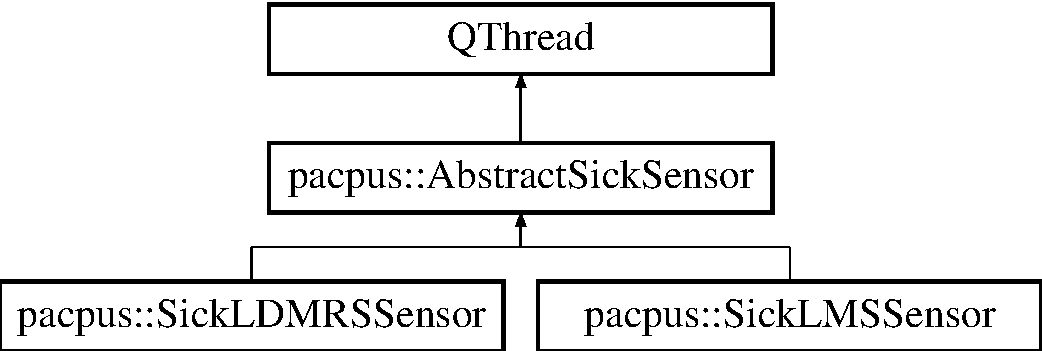
\includegraphics[height=3.000000cm]{classpacpus_1_1AbstractSickSensor}
\end{center}
\end{figure}
\subsection*{Public Slots}
\begin{DoxyCompactItemize}
\item 
virtual void \hyperlink{classpacpus_1_1AbstractSickSensor_a566931db0cd4e37110d60f3a25eb8de6}{custom\-Event} (Q\-Event $\ast$e)=0
\begin{DoxyCompactList}\small\item\em custom\-Event is a slot called when connected to a signal. \end{DoxyCompactList}\end{DoxyCompactItemize}
\subsection*{Public Member Functions}
\begin{DoxyCompactItemize}
\item 
\hypertarget{classpacpus_1_1AbstractSickSensor_ae0577b049c0ad3dd79f1d56bcc9f3fe2}{void {\bfseries run} ()}\label{classpacpus_1_1AbstractSickSensor_ae0577b049c0ad3dd79f1d56bcc9f3fe2}

\item 
virtual void \hyperlink{classpacpus_1_1AbstractSickSensor_a14c6da8df61d91f2b63439df00fd5d6a}{stop\-Activity} ()=0
\item 
virtual void \hyperlink{classpacpus_1_1AbstractSickSensor_af8e017866cf70db766dbd11b60a52425}{start\-Activity} ()=0
\end{DoxyCompactItemize}
\subsection*{Public Attributes}
\begin{DoxyCompactItemize}
\item 
\hypertarget{classpacpus_1_1AbstractSickSensor_af030c5aadd2868dc741b25ba1dc07f9f}{\hyperlink{classpacpus_1_1SickSocket}{Sick\-Socket} $\ast$ {\bfseries S\-\_\-socket}}\label{classpacpus_1_1AbstractSickSensor_af030c5aadd2868dc741b25ba1dc07f9f}

\end{DoxyCompactItemize}
\subsection*{Protected Attributes}
\begin{DoxyCompactItemize}
\item 
\hypertarget{classpacpus_1_1AbstractSickSensor_ab617c6d1973124fa26053c7b928920aa}{Q\-String \hyperlink{classpacpus_1_1AbstractSickSensor_ab617c6d1973124fa26053c7b928920aa}{host\-\_\-}}\label{classpacpus_1_1AbstractSickSensor_ab617c6d1973124fa26053c7b928920aa}

\begin{DoxyCompactList}\small\item\em The Sick\-L\-D\-M\-R\-S I\-P or hostname. \end{DoxyCompactList}\item 
\hypertarget{classpacpus_1_1AbstractSickSensor_a58a4923a77b6be4d5847837e57be3b76}{int \hyperlink{classpacpus_1_1AbstractSickSensor_a58a4923a77b6be4d5847837e57be3b76}{port\-\_\-}}\label{classpacpus_1_1AbstractSickSensor_a58a4923a77b6be4d5847837e57be3b76}

\begin{DoxyCompactList}\small\item\em The Sick\-L\-D\-M\-R\-S port. \end{DoxyCompactList}\item 
\hypertarget{classpacpus_1_1AbstractSickSensor_a2cefb63d92089cab86f874a3390acb28}{bool \hyperlink{classpacpus_1_1AbstractSickSensor_a2cefb63d92089cab86f874a3390acb28}{recording}}\label{classpacpus_1_1AbstractSickSensor_a2cefb63d92089cab86f874a3390acb28}

\begin{DoxyCompactList}\small\item\em If data need to be recorded, set this member to true. \end{DoxyCompactList}\end{DoxyCompactItemize}


\subsection{Detailed Description}
The \hyperlink{classpacpus_1_1AbstractSickSensor}{Abstract\-Sick\-Sensor} class. 

The \hyperlink{classpacpus_1_1AbstractSickSensor}{Abstract\-Sick\-Sensor} class provides the abstract model for implementing sensor interfaces using \hyperlink{classpacpus_1_1SickComponent}{Sick\-Component}, used with the P\-A\-C\-P\-U\-S Framework. 

\subsection{Member Function Documentation}
\hypertarget{classpacpus_1_1AbstractSickSensor_a566931db0cd4e37110d60f3a25eb8de6}{\index{pacpus\-::\-Abstract\-Sick\-Sensor@{pacpus\-::\-Abstract\-Sick\-Sensor}!custom\-Event@{custom\-Event}}
\index{custom\-Event@{custom\-Event}!pacpus::AbstractSickSensor@{pacpus\-::\-Abstract\-Sick\-Sensor}}
\subsubsection[{custom\-Event}]{\setlength{\rightskip}{0pt plus 5cm}virtual void pacpus\-::\-Abstract\-Sick\-Sensor\-::custom\-Event (
\begin{DoxyParamCaption}
\item[{Q\-Event $\ast$}]{e}
\end{DoxyParamCaption}
)\hspace{0.3cm}{\ttfamily [pure virtual]}, {\ttfamily [slot]}}}\label{classpacpus_1_1AbstractSickSensor_a566931db0cd4e37110d60f3a25eb8de6}


custom\-Event is a slot called when connected to a signal. 


\begin{DoxyParams}{Parameters}
{\em e} & Q\-Event that carries information from sensor.\\
\hline
\end{DoxyParams}
Sick sensor interface implementation uses this slot to get data from the remote sensor, using I\-P packets. As long as Sick sensors use T\-C\-P/\-I\-P interface, it is advised to use this slot to get the packets from the device. \begin{DoxySeeAlso}{See Also}
\hyperlink{classpacpus_1_1SickFrameEvent}{Sick\-Frame\-Event} 
\end{DoxySeeAlso}
\hypertarget{classpacpus_1_1AbstractSickSensor_af8e017866cf70db766dbd11b60a52425}{\index{pacpus\-::\-Abstract\-Sick\-Sensor@{pacpus\-::\-Abstract\-Sick\-Sensor}!start\-Activity@{start\-Activity}}
\index{start\-Activity@{start\-Activity}!pacpus::AbstractSickSensor@{pacpus\-::\-Abstract\-Sick\-Sensor}}
\subsubsection[{start\-Activity}]{\setlength{\rightskip}{0pt plus 5cm}virtual void pacpus\-::\-Abstract\-Sick\-Sensor\-::start\-Activity (
\begin{DoxyParamCaption}
{}
\end{DoxyParamCaption}
)\hspace{0.3cm}{\ttfamily [pure virtual]}}}\label{classpacpus_1_1AbstractSickSensor_af8e017866cf70db766dbd11b60a52425}
to start the processing thread 

Implemented in \hyperlink{classpacpus_1_1SickLDMRSSensor_a2b82c6f677fe7e7e712b7397fb5390ee}{pacpus\-::\-Sick\-L\-D\-M\-R\-S\-Sensor}, and \hyperlink{classpacpus_1_1SickLMSSensor_a6268a9b5b17db84b662c562ea332541f}{pacpus\-::\-Sick\-L\-M\-S\-Sensor}.

\hypertarget{classpacpus_1_1AbstractSickSensor_a14c6da8df61d91f2b63439df00fd5d6a}{\index{pacpus\-::\-Abstract\-Sick\-Sensor@{pacpus\-::\-Abstract\-Sick\-Sensor}!stop\-Activity@{stop\-Activity}}
\index{stop\-Activity@{stop\-Activity}!pacpus::AbstractSickSensor@{pacpus\-::\-Abstract\-Sick\-Sensor}}
\subsubsection[{stop\-Activity}]{\setlength{\rightskip}{0pt plus 5cm}virtual void pacpus\-::\-Abstract\-Sick\-Sensor\-::stop\-Activity (
\begin{DoxyParamCaption}
{}
\end{DoxyParamCaption}
)\hspace{0.3cm}{\ttfamily [pure virtual]}}}\label{classpacpus_1_1AbstractSickSensor_a14c6da8df61d91f2b63439df00fd5d6a}
to stop the processing thread 

Implemented in \hyperlink{classpacpus_1_1SickLDMRSSensor_a5b3674df80e98093692fac9643819ab5}{pacpus\-::\-Sick\-L\-D\-M\-R\-S\-Sensor}, and \hyperlink{classpacpus_1_1SickLMSSensor_a082417a753cef1d4f726c50b2e14a4d0}{pacpus\-::\-Sick\-L\-M\-S\-Sensor}.



The documentation for this class was generated from the following file\-:\begin{DoxyCompactItemize}
\item 
Abstract\-Sick\-Sensor.\-h\end{DoxyCompactItemize}

\hypertarget{structpacpus_1_1DataHeader}{\section{pacpus\-:\-:Data\-Header Struct Reference}
\label{structpacpus_1_1DataHeader}\index{pacpus\-::\-Data\-Header@{pacpus\-::\-Data\-Header}}
}


The \hyperlink{structpacpus_1_1DataHeader}{Data\-Header} struct.  




{\ttfamily \#include $<$Sick\-L\-D\-M\-R\-S\-Data.\-h$>$}

\subsection*{Public Attributes}
\begin{DoxyCompactItemize}
\item 
\hypertarget{structpacpus_1_1DataHeader_a98d42f04ff2e365418a3bd7310f6922e}{u\-\_\-int32\-\_\-t \hyperlink{structpacpus_1_1DataHeader_a98d42f04ff2e365418a3bd7310f6922e}{magic\-Word}}\label{structpacpus_1_1DataHeader_a98d42f04ff2e365418a3bd7310f6922e}

\begin{DoxyCompactList}\small\item\em 0x\-A\-F\-F\-E\-C0\-C2 for the Sick L\-D\-M\-R\-S sensor (this value must be found in order to decode the message). \end{DoxyCompactList}\item 
\hypertarget{structpacpus_1_1DataHeader_acfc8ced0fba207de34a1f7215d4a6cb5}{u\-\_\-int32\-\_\-t \hyperlink{structpacpus_1_1DataHeader_acfc8ced0fba207de34a1f7215d4a6cb5}{size\-Previous\-Message}}\label{structpacpus_1_1DataHeader_acfc8ced0fba207de34a1f7215d4a6cb5}

\begin{DoxyCompactList}\small\item\em Size in bytes of the previous message. \end{DoxyCompactList}\item 
\hypertarget{structpacpus_1_1DataHeader_a71a67d094751e3c5a9117d5df5e86f62}{u\-\_\-int32\-\_\-t \hyperlink{structpacpus_1_1DataHeader_a71a67d094751e3c5a9117d5df5e86f62}{size\-Current\-Message}}\label{structpacpus_1_1DataHeader_a71a67d094751e3c5a9117d5df5e86f62}

\begin{DoxyCompactList}\small\item\em Size of the message content without the header (\hyperlink{structpacpus_1_1DataHeader}{Data\-Header}). \end{DoxyCompactList}\item 
\hypertarget{structpacpus_1_1DataHeader_a15664fcb384de15a6507e4da57294781}{u\-\_\-int8\-\_\-t \hyperlink{structpacpus_1_1DataHeader_a15664fcb384de15a6507e4da57294781}{device\-Id}}\label{structpacpus_1_1DataHeader_a15664fcb384de15a6507e4da57294781}

\begin{DoxyCompactList}\small\item\em Unused in data received directly from L\-D-\/\-M\-R\-S sensors. \end{DoxyCompactList}\item 
u\-\_\-int16\-\_\-t \hyperlink{structpacpus_1_1DataHeader_a2e11011e26d0344376cb812b5b858a64}{data\-Type}
\item 
\hypertarget{structpacpus_1_1DataHeader_a2c9728a402325ccadd4c69f3854e9eef}{u\-\_\-int64\-\_\-t \hyperlink{structpacpus_1_1DataHeader_a2c9728a402325ccadd4c69f3854e9eef}{ntp\-Time}}\label{structpacpus_1_1DataHeader_a2c9728a402325ccadd4c69f3854e9eef}

\begin{DoxyCompactList}\small\item\em Time of the sensor when the message is created. \end{DoxyCompactList}\end{DoxyCompactItemize}


\subsection{Detailed Description}
The \hyperlink{structpacpus_1_1DataHeader}{Data\-Header} struct. 

The \hyperlink{structpacpus_1_1DataHeader}{Data\-Header} struct describes general information about the message used with. On Sick L\-D\-M\-R\-S, \hyperlink{structpacpus_1_1DataHeader}{Data\-Header} corresponds exactly to the very first data carried into the whole message. See \href{docs/BAMessdatenProtokoll_LDMRSen_8014492_20110601.pdf}{\tt Ethernet data protocol L\-D-\/\-M\-R\-S, page 4}. \begin{quotation}
Warning \-: the data from the sensor is coded in Big Endian format. \end{quotation}


\subsection{Member Data Documentation}
\hypertarget{structpacpus_1_1DataHeader_a2e11011e26d0344376cb812b5b858a64}{\index{pacpus\-::\-Data\-Header@{pacpus\-::\-Data\-Header}!data\-Type@{data\-Type}}
\index{data\-Type@{data\-Type}!pacpus::DataHeader@{pacpus\-::\-Data\-Header}}
\subsubsection[{data\-Type}]{\setlength{\rightskip}{0pt plus 5cm}u\-\_\-int16\-\_\-t pacpus\-::\-Data\-Header\-::data\-Type}}\label{structpacpus_1_1DataHeader_a2e11011e26d0344376cb812b5b858a64}
Type of information carried into the message. Types used are \-:
\begin{DoxyItemize}
\item Points \-: 0x2202
\item Objects \-: 0x2221 
\end{DoxyItemize}

The documentation for this struct was generated from the following file\-:\begin{DoxyCompactItemize}
\item 
Sick\-L\-D\-M\-R\-S\-Data.\-h\end{DoxyCompactItemize}

\hypertarget{classpacpus_1_1MessageLDMRS}{\section{pacpus\-:\-:Message\-L\-D\-M\-R\-S Class Reference}
\label{classpacpus_1_1MessageLDMRS}\index{pacpus\-::\-Message\-L\-D\-M\-R\-S@{pacpus\-::\-Message\-L\-D\-M\-R\-S}}
}


The class carrying Sick L\-D\-M\-R\-S message.  




{\ttfamily \#include $<$Sick\-L\-D\-M\-R\-S\-Sensor.\-h$>$}

\subsection*{Public Member Functions}
\begin{DoxyCompactItemize}
\item 
\hypertarget{classpacpus_1_1MessageLDMRS_a2f18d36d67deb2c4e77dbc476d68821c}{\hyperlink{classpacpus_1_1MessageLDMRS_a2f18d36d67deb2c4e77dbc476d68821c}{Message\-L\-D\-M\-R\-S} ()}\label{classpacpus_1_1MessageLDMRS_a2f18d36d67deb2c4e77dbc476d68821c}

\begin{DoxyCompactList}\small\item\em Constructor. \end{DoxyCompactList}\item 
\hypertarget{classpacpus_1_1MessageLDMRS_acf5ece71eb2e00750db5e57610eb4a66}{\hyperlink{classpacpus_1_1MessageLDMRS_acf5ece71eb2e00750db5e57610eb4a66}{$\sim$\-Message\-L\-D\-M\-R\-S} ()}\label{classpacpus_1_1MessageLDMRS_acf5ece71eb2e00750db5e57610eb4a66}

\begin{DoxyCompactList}\small\item\em Destructor. \end{DoxyCompactList}\end{DoxyCompactItemize}
\subsection*{Public Attributes}
\begin{DoxyCompactItemize}
\item 
\hypertarget{classpacpus_1_1MessageLDMRS_a0de8de7be8864e2eb153c1b58b597a86}{\hyperlink{structpacpus_1_1DataHeader}{Data\-Header} \hyperlink{classpacpus_1_1MessageLDMRS_a0de8de7be8864e2eb153c1b58b597a86}{h\-Data}}\label{classpacpus_1_1MessageLDMRS_a0de8de7be8864e2eb153c1b58b597a86}

\begin{DoxyCompactList}\small\item\em An instance of \hyperlink{structpacpus_1_1DataHeader}{Data\-Header}. \end{DoxyCompactList}\item 
\hypertarget{classpacpus_1_1MessageLDMRS_aa67a394ee95860cf887abb671b53fc8f}{\hyperlink{structpacpus_1_1ScanHeader}{Scan\-Header} \hyperlink{classpacpus_1_1MessageLDMRS_aa67a394ee95860cf887abb671b53fc8f}{h\-Scan}}\label{classpacpus_1_1MessageLDMRS_aa67a394ee95860cf887abb671b53fc8f}

\begin{DoxyCompactList}\small\item\em An instance of \hyperlink{structpacpus_1_1ScanHeader}{Scan\-Header} (if data type is scan points). \end{DoxyCompactList}\item 
char \hyperlink{classpacpus_1_1MessageLDMRS_ad4f54e3688d2cca3f9175b9622dbed24}{body} \mbox{[}B\-O\-D\-Y\-\_\-\-M\-A\-X\-\_\-\-S\-I\-Z\-E\mbox{]}
\begin{DoxyCompactList}\small\item\em An array of characters \-: raw data then array of points or objects, depending on data type. \end{DoxyCompactList}\item 
\hypertarget{classpacpus_1_1MessageLDMRS_adf281676d8146037ecf51805d0e6217e}{road\-\_\-time\-\_\-t \hyperlink{classpacpus_1_1MessageLDMRS_adf281676d8146037ecf51805d0e6217e}{time}}\label{classpacpus_1_1MessageLDMRS_adf281676d8146037ecf51805d0e6217e}

\begin{DoxyCompactList}\small\item\em Time when the message is received. \end{DoxyCompactList}\item 
\hypertarget{classpacpus_1_1MessageLDMRS_a3f6e1a477d895f8f9d228669f559cb2d}{road\-\_\-timerange\-\_\-t \hyperlink{classpacpus_1_1MessageLDMRS_a3f6e1a477d895f8f9d228669f559cb2d}{timerange}}\label{classpacpus_1_1MessageLDMRS_a3f6e1a477d895f8f9d228669f559cb2d}

\begin{DoxyCompactList}\small\item\em Timerange \-: roughly, time between measurement of a point and the processing step (not implemented). \end{DoxyCompactList}\end{DoxyCompactItemize}


\subsection{Detailed Description}
The class carrying Sick L\-D\-M\-R\-S message. 

This class is used so that we can store every information sent by a Sick L\-D\-M\-R\-S sensor. First, the raw data is stored in {\ttfamily body}. These data are then decoded and general information about the message is stored in \hyperlink{structpacpus_1_1DataHeader}{Data\-Header} and \hyperlink{structpacpus_1_1ScanHeader}{Scan\-Header} (Object data decoding is not implemented yet). Then, the body field is replaced by a \hyperlink{structpacpus_1_1ScanPoint}{Scan\-Point} or \hyperlink{structpacpus_1_1ScanObject}{Scan\-Object} array in order to be stored in D\-B\-T/\-U\-T\-C files. 

\subsection{Member Data Documentation}
\hypertarget{classpacpus_1_1MessageLDMRS_ad4f54e3688d2cca3f9175b9622dbed24}{\index{pacpus\-::\-Message\-L\-D\-M\-R\-S@{pacpus\-::\-Message\-L\-D\-M\-R\-S}!body@{body}}
\index{body@{body}!pacpus::MessageLDMRS@{pacpus\-::\-Message\-L\-D\-M\-R\-S}}
\subsubsection[{body}]{\setlength{\rightskip}{0pt plus 5cm}char pacpus\-::\-Message\-L\-D\-M\-R\-S\-::body\mbox{[}B\-O\-D\-Y\-\_\-\-M\-A\-X\-\_\-\-S\-I\-Z\-E\mbox{]}}}\label{classpacpus_1_1MessageLDMRS_ad4f54e3688d2cca3f9175b9622dbed24}


An array of characters \-: raw data then array of points or objects, depending on data type. 

This array pointer points to allocated in memory (basically, in heap (malloc)) and then must be freed (free) when the whole message is decoded and stored. 

The documentation for this class was generated from the following file\-:\begin{DoxyCompactItemize}
\item 
Sick\-L\-D\-M\-R\-S\-Sensor.\-h\end{DoxyCompactItemize}

\hypertarget{classpacpus_1_1MessageLMS}{\section{pacpus\-:\-:Message\-L\-M\-S Class Reference}
\label{classpacpus_1_1MessageLMS}\index{pacpus\-::\-Message\-L\-M\-S@{pacpus\-::\-Message\-L\-M\-S}}
}


The class carrying Sick L\-M\-S message.  




{\ttfamily \#include $<$Sick\-L\-M\-S\-Sensor.\-h$>$}

\subsection*{Public Member Functions}
\begin{DoxyCompactItemize}
\item 
\hypertarget{classpacpus_1_1MessageLMS_a20ef9a5b76448142f0bf88a859c5d042}{\hyperlink{classpacpus_1_1MessageLMS_a20ef9a5b76448142f0bf88a859c5d042}{Message\-L\-M\-S} ()}\label{classpacpus_1_1MessageLMS_a20ef9a5b76448142f0bf88a859c5d042}

\begin{DoxyCompactList}\small\item\em Constructor. \end{DoxyCompactList}\item 
\hypertarget{classpacpus_1_1MessageLMS_a586746e0e35aa83419044efd92556ea4}{\hyperlink{classpacpus_1_1MessageLMS_a586746e0e35aa83419044efd92556ea4}{$\sim$\-Message\-L\-M\-S} ()}\label{classpacpus_1_1MessageLMS_a586746e0e35aa83419044efd92556ea4}

\begin{DoxyCompactList}\small\item\em Destructor. \end{DoxyCompactList}\end{DoxyCompactItemize}
\subsection*{Public Attributes}
\begin{DoxyCompactItemize}
\item 
\hypertarget{classpacpus_1_1MessageLMS_a5448754297046a46de36a32e8500f93e}{\hyperlink{structpacpus_1_1__scanData}{scan\-Data} \hyperlink{classpacpus_1_1MessageLMS_a5448754297046a46de36a32e8500f93e}{data}}\label{classpacpus_1_1MessageLMS_a5448754297046a46de36a32e8500f93e}

\begin{DoxyCompactList}\small\item\em Every needed information about the scan (general info + scan points). \end{DoxyCompactList}\item 
\hypertarget{classpacpus_1_1MessageLMS_a6b8f1da7a50fae0c3d1b4adeec39eff7}{long \hyperlink{classpacpus_1_1MessageLMS_a6b8f1da7a50fae0c3d1b4adeec39eff7}{msg\-Size}}\label{classpacpus_1_1MessageLMS_a6b8f1da7a50fae0c3d1b4adeec39eff7}

\begin{DoxyCompactList}\small\item\em Size of the message. \end{DoxyCompactList}\item 
\hypertarget{classpacpus_1_1MessageLMS_a7570d407b4cdac7450adde9448b231ae}{std\-::vector$<$ std\-::string $>$ $\ast$ \hyperlink{classpacpus_1_1MessageLMS_a7570d407b4cdac7450adde9448b231ae}{split\-Message}}\label{classpacpus_1_1MessageLMS_a7570d407b4cdac7450adde9448b231ae}

\begin{DoxyCompactList}\small\item\em The message is split into an array of string in order to be processed easily. \end{DoxyCompactList}\item 
\hypertarget{classpacpus_1_1MessageLMS_a87494c8ed7daece40f1456a0b028990a}{char $\ast$ \hyperlink{classpacpus_1_1MessageLMS_a87494c8ed7daece40f1456a0b028990a}{body}}\label{classpacpus_1_1MessageLMS_a87494c8ed7daece40f1456a0b028990a}

\begin{DoxyCompactList}\small\item\em Raw data. \end{DoxyCompactList}\item 
\hypertarget{classpacpus_1_1MessageLMS_a3b81e17d0f28e13933e50337dcf5e45b}{road\-\_\-time\-\_\-t \hyperlink{classpacpus_1_1MessageLMS_a3b81e17d0f28e13933e50337dcf5e45b}{time}}\label{classpacpus_1_1MessageLMS_a3b81e17d0f28e13933e50337dcf5e45b}

\begin{DoxyCompactList}\small\item\em Time when the first packet of the message is received. \end{DoxyCompactList}\item 
\hypertarget{classpacpus_1_1MessageLMS_ab2158c796fc5510232ed9a222264f899}{road\-\_\-timerange\-\_\-t \hyperlink{classpacpus_1_1MessageLMS_ab2158c796fc5510232ed9a222264f899}{timerange}}\label{classpacpus_1_1MessageLMS_ab2158c796fc5510232ed9a222264f899}

\begin{DoxyCompactList}\small\item\em Timerange \-: roughly, time between measurement of a point and the processing step (not implemented). \end{DoxyCompactList}\end{DoxyCompactItemize}


\subsection{Detailed Description}
The class carrying Sick L\-M\-S message. 

This class is used so that we can store every information sent by a Sick L\-M\-S sensor. First, the raw data is stored in {\ttfamily body}. Then, if the message is relevant, {\ttfamily split\-Message} is instanciated in order to parse easily information from the sensor. These data are then decoded and stored in the scan\-Data structure. 

The documentation for this class was generated from the following file\-:\begin{DoxyCompactItemize}
\item 
Sick\-L\-M\-S\-Sensor.\-h\end{DoxyCompactItemize}

\hypertarget{structpacpus_1_1MessagePacket}{\section{pacpus\-:\-:Message\-Packet Struct Reference}
\label{structpacpus_1_1MessagePacket}\index{pacpus\-::\-Message\-Packet@{pacpus\-::\-Message\-Packet}}
}


Structure used to stored Sick data between several decoding processes.  




{\ttfamily \#include $<$Abstract\-Sick\-Sensor.\-h$>$}

\subsection*{Public Attributes}
\begin{DoxyCompactItemize}
\item 
\hypertarget{structpacpus_1_1MessagePacket_a8662b64b5eba2ca27aeba340e79a47c9}{road\-\_\-time\-\_\-t {\bfseries time}}\label{structpacpus_1_1MessagePacket_a8662b64b5eba2ca27aeba340e79a47c9}

\item 
\hypertarget{structpacpus_1_1MessagePacket_afcacd2d4d236410ad9352050e42346e7}{std\-::string {\bfseries data}}\label{structpacpus_1_1MessagePacket_afcacd2d4d236410ad9352050e42346e7}

\item 
\hypertarget{structpacpus_1_1MessagePacket_afd653684969f8d6f68564559d82b7241}{bool {\bfseries previous\-Data}}\label{structpacpus_1_1MessagePacket_afd653684969f8d6f68564559d82b7241}

\end{DoxyCompactItemize}


\subsection{Detailed Description}
Structure used to stored Sick data between several decoding processes. 

Note that data coming from sensors are split in I\-P packets. In order to get the whole message in one block, \hyperlink{structpacpus_1_1MessagePacket}{Message\-Packet} is used to reconstitue the raw data. As we want to reconstitute the message, it is useful to know if another packet belonging to the message was previously received. Also, the time of the reception of the first packet is carried into the structure in order to trace scans. 

The documentation for this struct was generated from the following file\-:\begin{DoxyCompactItemize}
\item 
Abstract\-Sick\-Sensor.\-h\end{DoxyCompactItemize}

\hypertarget{structpacpus_1_1ScanHeader}{\section{pacpus\-:\-:Scan\-Header Struct Reference}
\label{structpacpus_1_1ScanHeader}\index{pacpus\-::\-Scan\-Header@{pacpus\-::\-Scan\-Header}}
}


The \hyperlink{structpacpus_1_1ScanHeader}{Scan\-Header} struct.  




{\ttfamily \#include $<$Sick\-L\-D\-M\-R\-S\-Data.\-h$>$}

\subsection*{Public Attributes}
\begin{DoxyCompactItemize}
\item 
\hypertarget{structpacpus_1_1ScanHeader_a1cf721c87e6bf8c022dc134bc1a861f1}{u\-\_\-int16\-\_\-t \hyperlink{structpacpus_1_1ScanHeader_a1cf721c87e6bf8c022dc134bc1a861f1}{scan\-Number}}\label{structpacpus_1_1ScanHeader_a1cf721c87e6bf8c022dc134bc1a861f1}

\begin{DoxyCompactList}\small\item\em Number of the scan since the sensor started measuring. \end{DoxyCompactList}\item 
u\-\_\-int16\-\_\-t \hyperlink{structpacpus_1_1ScanHeader_aad5f68bdf71fe32c0325f69919355aa7}{scanner\-Status}
\begin{DoxyCompactList}\small\item\em Status of the scanner. \end{DoxyCompactList}\item 
\hypertarget{structpacpus_1_1ScanHeader_a55369f8979b18292592fe7e63538e8b0}{u\-\_\-int16\-\_\-t {\bfseries phase\-Offset}}\label{structpacpus_1_1ScanHeader_a55369f8979b18292592fe7e63538e8b0}

\item 
\hypertarget{structpacpus_1_1ScanHeader_a498752799f73dcdea074bb346be9c909}{u\-\_\-int64\-\_\-t \hyperlink{structpacpus_1_1ScanHeader_a498752799f73dcdea074bb346be9c909}{start\-Ntp\-Time}}\label{structpacpus_1_1ScanHeader_a498752799f73dcdea074bb346be9c909}

\begin{DoxyCompactList}\small\item\em N\-T\-P time first measurement. \end{DoxyCompactList}\item 
\hypertarget{structpacpus_1_1ScanHeader_a9383aebf0708f9608d2ee0a0b4cb8c28}{u\-\_\-int64\-\_\-t \hyperlink{structpacpus_1_1ScanHeader_a9383aebf0708f9608d2ee0a0b4cb8c28}{end\-Ntp\-Time}}\label{structpacpus_1_1ScanHeader_a9383aebf0708f9608d2ee0a0b4cb8c28}

\begin{DoxyCompactList}\small\item\em N\-T\-P time last measurement. \end{DoxyCompactList}\item 
\hypertarget{structpacpus_1_1ScanHeader_ae90050c5f517aab0ddec6a0a7a905e97}{u\-\_\-int16\-\_\-t \hyperlink{structpacpus_1_1ScanHeader_ae90050c5f517aab0ddec6a0a7a905e97}{ticks\-Per\-Rot}}\label{structpacpus_1_1ScanHeader_ae90050c5f517aab0ddec6a0a7a905e97}

\begin{DoxyCompactList}\small\item\em Angle ticks per rotation (used to compute the real angle of a point) \end{DoxyCompactList}\item 
\hypertarget{structpacpus_1_1ScanHeader_a805ffbef47d7e001ec4d22b8a56afd87}{int16\-\_\-t \hyperlink{structpacpus_1_1ScanHeader_a805ffbef47d7e001ec4d22b8a56afd87}{start\-Angle}}\label{structpacpus_1_1ScanHeader_a805ffbef47d7e001ec4d22b8a56afd87}

\begin{DoxyCompactList}\small\item\em Angle of the first measured value. \end{DoxyCompactList}\item 
\hypertarget{structpacpus_1_1ScanHeader_ab7342b6eb6939702c6a2d0f61cd212d8}{int16\-\_\-t \hyperlink{structpacpus_1_1ScanHeader_ab7342b6eb6939702c6a2d0f61cd212d8}{end\-Angle}}\label{structpacpus_1_1ScanHeader_ab7342b6eb6939702c6a2d0f61cd212d8}

\begin{DoxyCompactList}\small\item\em Angle of the last measured value. \end{DoxyCompactList}\item 
u\-\_\-int16\-\_\-t \hyperlink{structpacpus_1_1ScanHeader_a92f397bf893b9869c8847eb4a39a8005}{num\-Points}
\begin{DoxyCompactList}\small\item\em Number of scanned points during this scan. \end{DoxyCompactList}\end{DoxyCompactItemize}


\subsection{Detailed Description}
The \hyperlink{structpacpus_1_1ScanHeader}{Scan\-Header} struct. 

General information about points measured. Data type is 0x2202 \begin{DoxySeeAlso}{See Also}
\hyperlink{structpacpus_1_1DataHeader}{Data\-Header}
\end{DoxySeeAlso}
see Ethernet data protocol L\-D-\/\-M\-R\-S page 5 

\subsection{Member Data Documentation}
\hypertarget{structpacpus_1_1ScanHeader_a92f397bf893b9869c8847eb4a39a8005}{\index{pacpus\-::\-Scan\-Header@{pacpus\-::\-Scan\-Header}!num\-Points@{num\-Points}}
\index{num\-Points@{num\-Points}!pacpus::ScanHeader@{pacpus\-::\-Scan\-Header}}
\subsubsection[{num\-Points}]{\setlength{\rightskip}{0pt plus 5cm}u\-\_\-int16\-\_\-t pacpus\-::\-Scan\-Header\-::num\-Points}}\label{structpacpus_1_1ScanHeader_a92f397bf893b9869c8847eb4a39a8005}


Number of scanned points during this scan. 

\begin{DoxySeeAlso}{See Also}
\hyperlink{structpacpus_1_1ScanPoint}{Scan\-Point} 
\end{DoxySeeAlso}
\hypertarget{structpacpus_1_1ScanHeader_aad5f68bdf71fe32c0325f69919355aa7}{\index{pacpus\-::\-Scan\-Header@{pacpus\-::\-Scan\-Header}!scanner\-Status@{scanner\-Status}}
\index{scanner\-Status@{scanner\-Status}!pacpus::ScanHeader@{pacpus\-::\-Scan\-Header}}
\subsubsection[{scanner\-Status}]{\setlength{\rightskip}{0pt plus 5cm}u\-\_\-int16\-\_\-t pacpus\-::\-Scan\-Header\-::scanner\-Status}}\label{structpacpus_1_1ScanHeader_aad5f68bdf71fe32c0325f69919355aa7}


Status of the scanner. 


\begin{DoxyItemize}
\item 0x0007\-: reserved,
\item 0x0008\-: set frequency reached,
\item 0x0010\-: external sync signal detected,
\item 0x0020\-: sync ok,
\item 0x0040\-: sync master (instead of slave),
\item 0x\-F\-F80\-: reserved 
\end{DoxyItemize}

The documentation for this struct was generated from the following file\-:\begin{DoxyCompactItemize}
\item 
Sick\-L\-D\-M\-R\-S\-Data.\-h\end{DoxyCompactItemize}

\hypertarget{structpacpus_1_1ScanObject}{\section{pacpus\-:\-:Scan\-Object Struct Reference}
\label{structpacpus_1_1ScanObject}\index{pacpus\-::\-Scan\-Object@{pacpus\-::\-Scan\-Object}}
}


The \hyperlink{structpacpus_1_1ScanObject}{Scan\-Object} struct (not used)  




{\ttfamily \#include $<$Sick\-L\-D\-M\-R\-S\-Data.\-h$>$}



\subsection{Detailed Description}
The \hyperlink{structpacpus_1_1ScanObject}{Scan\-Object} struct (not used) 

Used to describe an object. Data type 0x2221 \begin{DoxySeeAlso}{See Also}
\hyperlink{structpacpus_1_1DataHeader}{Data\-Header} 
\end{DoxySeeAlso}


The documentation for this struct was generated from the following file\-:\begin{DoxyCompactItemize}
\item 
Sick\-L\-D\-M\-R\-S\-Data.\-h\end{DoxyCompactItemize}

\hypertarget{structpacpus_1_1ScanPoint}{\section{pacpus\-:\-:Scan\-Point Struct Reference}
\label{structpacpus_1_1ScanPoint}\index{pacpus\-::\-Scan\-Point@{pacpus\-::\-Scan\-Point}}
}


The \hyperlink{structpacpus_1_1ScanPoint}{Scan\-Point} struct.  




{\ttfamily \#include $<$Sick\-L\-D\-M\-R\-S\-Data.\-h$>$}

\subsection*{Public Attributes}
\begin{DoxyCompactItemize}
\item 
u\-\_\-char \hyperlink{structpacpus_1_1ScanPoint_a300ce0213fd1a9ea59687f29b68046bc}{layer\-Echo}
\item 
\hypertarget{structpacpus_1_1ScanPoint_a6a3519e30743dee6230e7167f4c250f3}{u\-\_\-char {\bfseries flags}}\label{structpacpus_1_1ScanPoint_a6a3519e30743dee6230e7167f4c250f3}

\item 
u\-\_\-int16\-\_\-t \hyperlink{structpacpus_1_1ScanPoint_af551038f4f967b5289f50c9454bc8619}{angle}
\item 
\hypertarget{structpacpus_1_1ScanPoint_a74e9ebbf0df0e334e74788ce34410f80}{u\-\_\-int16\-\_\-t \hyperlink{structpacpus_1_1ScanPoint_a74e9ebbf0df0e334e74788ce34410f80}{distance}}\label{structpacpus_1_1ScanPoint_a74e9ebbf0df0e334e74788ce34410f80}

\begin{DoxyCompactList}\small\item\em Distance of the point from the sensor in centimeters. \end{DoxyCompactList}\item 
\hypertarget{structpacpus_1_1ScanPoint_a8c32bbdc82afbd32100ceb959eb645d7}{u\-\_\-int16\-\_\-t \hyperlink{structpacpus_1_1ScanPoint_a8c32bbdc82afbd32100ceb959eb645d7}{echo\-Pulse\-Width}}\label{structpacpus_1_1ScanPoint_a8c32bbdc82afbd32100ceb959eb645d7}

\begin{DoxyCompactList}\small\item\em Width of echo pulse (cm) \end{DoxyCompactList}\end{DoxyCompactItemize}


\subsection{Detailed Description}
The \hyperlink{structpacpus_1_1ScanPoint}{Scan\-Point} struct. 

Used to describe a point. Data type 0x2202\begin{DoxySeeAlso}{See Also}
\hyperlink{structpacpus_1_1DataHeader}{Data\-Header} 
\end{DoxySeeAlso}


\subsection{Member Data Documentation}
\hypertarget{structpacpus_1_1ScanPoint_af551038f4f967b5289f50c9454bc8619}{\index{pacpus\-::\-Scan\-Point@{pacpus\-::\-Scan\-Point}!angle@{angle}}
\index{angle@{angle}!pacpus::ScanPoint@{pacpus\-::\-Scan\-Point}}
\subsubsection[{angle}]{\setlength{\rightskip}{0pt plus 5cm}u\-\_\-int16\-\_\-t pacpus\-::\-Scan\-Point\-::angle}}\label{structpacpus_1_1ScanPoint_af551038f4f967b5289f50c9454bc8619}
Angle in number of ticks. You can easily compute the real angle \-: $ angle (degree) = \frac{angle (ticks)}{ScanHeader.ticksPerRot}$\begin{DoxySeeAlso}{See Also}
\hyperlink{structpacpus_1_1ScanHeader}{Scan\-Header} 
\end{DoxySeeAlso}
\hypertarget{structpacpus_1_1ScanPoint_a300ce0213fd1a9ea59687f29b68046bc}{\index{pacpus\-::\-Scan\-Point@{pacpus\-::\-Scan\-Point}!layer\-Echo@{layer\-Echo}}
\index{layer\-Echo@{layer\-Echo}!pacpus::ScanPoint@{pacpus\-::\-Scan\-Point}}
\subsubsection[{layer\-Echo}]{\setlength{\rightskip}{0pt plus 5cm}u\-\_\-char pacpus\-::\-Scan\-Point\-::layer\-Echo}}\label{structpacpus_1_1ScanPoint_a300ce0213fd1a9ea59687f29b68046bc}
4 L\-S\-B \-: Layer (scan layer of the point) 4 M\-S\-B \-: Echo 

The documentation for this struct was generated from the following file\-:\begin{DoxyCompactItemize}
\item 
Sick\-L\-D\-M\-R\-S\-Data.\-h\end{DoxyCompactItemize}

\hypertarget{classpacpus_1_1SickComponent}{\section{pacpus\-:\-:Sick\-Component Class Reference}
\label{classpacpus_1_1SickComponent}\index{pacpus\-::\-Sick\-Component@{pacpus\-::\-Sick\-Component}}
}


The \hyperlink{classpacpus_1_1SickComponent}{Sick\-Component} class.  




{\ttfamily \#include $<$Sick\-Component.\-h$>$}

Inheritance diagram for pacpus\-:\-:Sick\-Component\-:\begin{figure}[H]
\begin{center}
\leavevmode
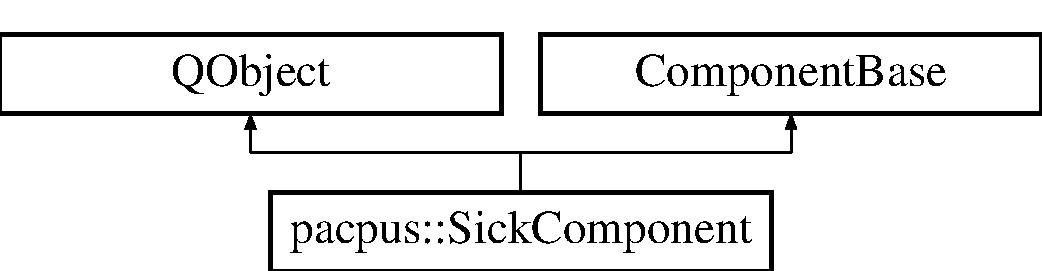
\includegraphics[height=2.000000cm]{classpacpus_1_1SickComponent}
\end{center}
\end{figure}
\subsection*{Public Member Functions}
\begin{DoxyCompactItemize}
\item 
\hypertarget{classpacpus_1_1SickComponent_a173293f307240ec6872d5be9a8790c56}{\hyperlink{classpacpus_1_1SickComponent_a173293f307240ec6872d5be9a8790c56}{Sick\-Component} (Q\-String name)}\label{classpacpus_1_1SickComponent_a173293f307240ec6872d5be9a8790c56}

\begin{DoxyCompactList}\small\item\em Constructor. \end{DoxyCompactList}\item 
\hypertarget{classpacpus_1_1SickComponent_a318cc1a398812c71a47661b22ff36e22}{\hyperlink{classpacpus_1_1SickComponent_a318cc1a398812c71a47661b22ff36e22}{$\sim$\-Sick\-Component} ()}\label{classpacpus_1_1SickComponent_a318cc1a398812c71a47661b22ff36e22}

\begin{DoxyCompactList}\small\item\em Destructor. \end{DoxyCompactList}\item 
virtual void \hyperlink{classpacpus_1_1SickComponent_a4524cb582e5fdf9dbd059072bea0d49b}{stop\-Activity} ()
\item 
virtual void \hyperlink{classpacpus_1_1SickComponent_a93980139bab330f3ef6bf818afba70a2}{start\-Activity} ()
\item 
virtual \\*
Component\-Base\-::\-C\-O\-M\-P\-O\-N\-E\-N\-T\-\_\-\-C\-O\-N\-F\-I\-G\-U\-R\-A\-T\-I\-O\-N \hyperlink{classpacpus_1_1SickComponent_accc413cdd2c4f5b8aacb14655b8a86d2}{configure\-Component} (Xml\-Component\-Config config)
\begin{DoxyCompactList}\small\item\em Configure compenent. \end{DoxyCompactList}\end{DoxyCompactItemize}
\subsection*{Public Attributes}
\begin{DoxyCompactItemize}
\item 
\hypertarget{classpacpus_1_1SickComponent_a4ac4764e115fb41e6e9df77e05bcb14f}{\hyperlink{classpacpus_1_1SickComponent}{Sick\-Component} $\ast$ {\bfseries my\-Parent}}\label{classpacpus_1_1SickComponent_a4ac4764e115fb41e6e9df77e05bcb14f}

\end{DoxyCompactItemize}


\subsection{Detailed Description}
The \hyperlink{classpacpus_1_1SickComponent}{Sick\-Component} class. 

This class defines a P\-A\-C\-P\-U\-S component used to acquire Sick lidars data. 

\subsection{Member Function Documentation}
\hypertarget{classpacpus_1_1SickComponent_accc413cdd2c4f5b8aacb14655b8a86d2}{\index{pacpus\-::\-Sick\-Component@{pacpus\-::\-Sick\-Component}!configure\-Component@{configure\-Component}}
\index{configure\-Component@{configure\-Component}!pacpus::SickComponent@{pacpus\-::\-Sick\-Component}}
\subsubsection[{configure\-Component}]{\setlength{\rightskip}{0pt plus 5cm}Component\-Base\-::\-C\-O\-M\-P\-O\-N\-E\-N\-T\-\_\-\-C\-O\-N\-F\-I\-G\-U\-R\-A\-T\-I\-O\-N pacpus\-::\-Sick\-Component\-::configure\-Component (
\begin{DoxyParamCaption}
\item[{Xml\-Component\-Config}]{config}
\end{DoxyParamCaption}
)\hspace{0.3cm}{\ttfamily [virtual]}}}\label{classpacpus_1_1SickComponent_accc413cdd2c4f5b8aacb14655b8a86d2}


Configure compenent. 


\begin{DoxyParams}{Parameters}
{\em config} & X\-M\-L file passed in order to configure the Sick Component.\\
\hline
\end{DoxyParams}
This function instanciate every sensors configured through the X\-M\-L file. The X\-M\-L file must be formated as expected by this function. Depending on used sensors and how many, you should define these three property in a \char`\"{}\-Sick\char`\"{} node (X must start from '0') \-:
\begin{DoxyItemize}
\item sickldmrs\-\_\-\-X
\item sicklms151\-\_\-\-X
\item sicklms511\-\_\-\-X
\end{DoxyItemize}

For example, let's say we have two Sick L\-M\-S151, one L\-D\-M\-R\-S and one L\-M\-S511 \-:

{\ttfamily  $<$\-Sick type=\char`\"{}\-Sick\-Component\char`\"{} sickldmrs\-\_\-0=\char`\"{}192.\-168.\-0.\-1\-:2111\char`\"{} sicklms151\-\_\-0=\char`\"{}192.\-168.\-0.\-10\-:2111\char`\"{} sicklms151\-\_\-1=\char`\"{}192.\-168.\-0.\-11\-:2111\char`\"{} sicklms511\-\_\-0=\char`\"{}192.\-168.\-1.\-50\-:2111\char`\"{}$>$ }

Do not forget {\ttfamily type=\char`\"{}\-Sick\-Component\char`\"{}}. \hypertarget{classpacpus_1_1SickComponent_a93980139bab330f3ef6bf818afba70a2}{\index{pacpus\-::\-Sick\-Component@{pacpus\-::\-Sick\-Component}!start\-Activity@{start\-Activity}}
\index{start\-Activity@{start\-Activity}!pacpus::SickComponent@{pacpus\-::\-Sick\-Component}}
\subsubsection[{start\-Activity}]{\setlength{\rightskip}{0pt plus 5cm}void pacpus\-::\-Sick\-Component\-::start\-Activity (
\begin{DoxyParamCaption}
{}
\end{DoxyParamCaption}
)\hspace{0.3cm}{\ttfamily [virtual]}}}\label{classpacpus_1_1SickComponent_a93980139bab330f3ef6bf818afba70a2}
To start the processing thread \hypertarget{classpacpus_1_1SickComponent_a4524cb582e5fdf9dbd059072bea0d49b}{\index{pacpus\-::\-Sick\-Component@{pacpus\-::\-Sick\-Component}!stop\-Activity@{stop\-Activity}}
\index{stop\-Activity@{stop\-Activity}!pacpus::SickComponent@{pacpus\-::\-Sick\-Component}}
\subsubsection[{stop\-Activity}]{\setlength{\rightskip}{0pt plus 5cm}void pacpus\-::\-Sick\-Component\-::stop\-Activity (
\begin{DoxyParamCaption}
{}
\end{DoxyParamCaption}
)\hspace{0.3cm}{\ttfamily [virtual]}}}\label{classpacpus_1_1SickComponent_a4524cb582e5fdf9dbd059072bea0d49b}
To stop the processing thread 

The documentation for this class was generated from the following files\-:\begin{DoxyCompactItemize}
\item 
Sick\-Component.\-h\item 
Sick\-Component.\-cpp\end{DoxyCompactItemize}

\hypertarget{classpacpus_1_1SickFrame}{\section{pacpus\-:\-:Sick\-Frame Class Reference}
\label{classpacpus_1_1SickFrame}\index{pacpus\-::\-Sick\-Frame@{pacpus\-::\-Sick\-Frame}}
}


The \hyperlink{classpacpus_1_1SickFrame}{Sick\-Frame} class.  




{\ttfamily \#include $<$Sick\-Socket.\-h$>$}

\subsection*{Public Member Functions}
\begin{DoxyCompactItemize}
\item 
\hypertarget{classpacpus_1_1SickFrame_ac579d615e5d5a5655cf77db24e05a4e2}{\hyperlink{classpacpus_1_1SickFrame_ac579d615e5d5a5655cf77db24e05a4e2}{Sick\-Frame} ()}\label{classpacpus_1_1SickFrame_ac579d615e5d5a5655cf77db24e05a4e2}

\begin{DoxyCompactList}\small\item\em \hyperlink{classpacpus_1_1SickFrame}{Sick\-Frame} constructor. \end{DoxyCompactList}\item 
\hypertarget{classpacpus_1_1SickFrame_a1836cf6f51350adccf73116096cd5a7a}{\hyperlink{classpacpus_1_1SickFrame_a1836cf6f51350adccf73116096cd5a7a}{$\sim$\-Sick\-Frame} ()}\label{classpacpus_1_1SickFrame_a1836cf6f51350adccf73116096cd5a7a}

\begin{DoxyCompactList}\small\item\em Destructor. \end{DoxyCompactList}\end{DoxyCompactItemize}
\subsection*{Public Attributes}
\begin{DoxyCompactItemize}
\item 
\hypertarget{classpacpus_1_1SickFrame_a80b987f69b595a40effddea23d620224}{qint64 \hyperlink{classpacpus_1_1SickFrame_a80b987f69b595a40effddea23d620224}{size}}\label{classpacpus_1_1SickFrame_a80b987f69b595a40effddea23d620224}

\begin{DoxyCompactList}\small\item\em Size of incoming packet. \end{DoxyCompactList}\item 
\hypertarget{classpacpus_1_1SickFrame_af0ed21fe9690c564356838543a3b0126}{road\-\_\-time\-\_\-t \hyperlink{classpacpus_1_1SickFrame_af0ed21fe9690c564356838543a3b0126}{time}}\label{classpacpus_1_1SickFrame_af0ed21fe9690c564356838543a3b0126}

\begin{DoxyCompactList}\small\item\em Time when packet is received. \end{DoxyCompactList}\item 
\hypertarget{classpacpus_1_1SickFrame_aeaaccfb07a72aae9306c16c5574950ca}{char $\ast$ \hyperlink{classpacpus_1_1SickFrame_aeaaccfb07a72aae9306c16c5574950ca}{msg}}\label{classpacpus_1_1SickFrame_aeaaccfb07a72aae9306c16c5574950ca}

\begin{DoxyCompactList}\small\item\em Packet (raw data). \end{DoxyCompactList}\end{DoxyCompactItemize}


\subsection{Detailed Description}
The \hyperlink{classpacpus_1_1SickFrame}{Sick\-Frame} class. 

The documentation for this class was generated from the following file\-:\begin{DoxyCompactItemize}
\item 
Sick\-Socket.\-h\end{DoxyCompactItemize}

\hypertarget{classpacpus_1_1SickFrameEvent}{\section{pacpus\-:\-:Sick\-Frame\-Event Class Reference}
\label{classpacpus_1_1SickFrameEvent}\index{pacpus\-::\-Sick\-Frame\-Event@{pacpus\-::\-Sick\-Frame\-Event}}
}


The \hyperlink{classpacpus_1_1SickFrameEvent}{Sick\-Frame\-Event} class Q\-Event that encapsulates packets.  




{\ttfamily \#include $<$Sick\-Socket.\-h$>$}

Inheritance diagram for pacpus\-:\-:Sick\-Frame\-Event\-:\begin{figure}[H]
\begin{center}
\leavevmode
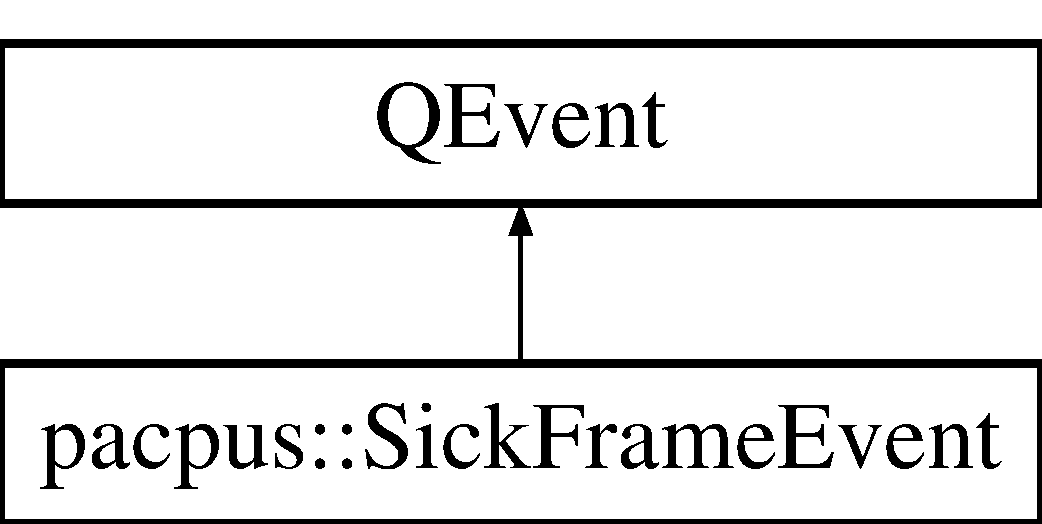
\includegraphics[height=2.000000cm]{classpacpus_1_1SickFrameEvent}
\end{center}
\end{figure}
\subsection*{Public Member Functions}
\begin{DoxyCompactItemize}
\item 
\hypertarget{classpacpus_1_1SickFrameEvent_a505ccae5cb63fee4ac3e30c8dbcc790b}{\hyperlink{classpacpus_1_1SickFrameEvent_a505ccae5cb63fee4ac3e30c8dbcc790b}{Sick\-Frame\-Event} ()}\label{classpacpus_1_1SickFrameEvent_a505ccae5cb63fee4ac3e30c8dbcc790b}

\begin{DoxyCompactList}\small\item\em Constructor. \end{DoxyCompactList}\item 
\hypertarget{classpacpus_1_1SickFrameEvent_a3028129c6245ac577323aa511be2b3a1}{\hyperlink{classpacpus_1_1SickFrameEvent_a3028129c6245ac577323aa511be2b3a1}{$\sim$\-Sick\-Frame\-Event} ()}\label{classpacpus_1_1SickFrameEvent_a3028129c6245ac577323aa511be2b3a1}

\begin{DoxyCompactList}\small\item\em Destructor. \end{DoxyCompactList}\end{DoxyCompactItemize}
\subsection*{Public Attributes}
\begin{DoxyCompactItemize}
\item 
\hypertarget{classpacpus_1_1SickFrameEvent_a8d27195b76d8c8d403c0e139347985aa}{\hyperlink{classpacpus_1_1SickFrame}{Sick\-Frame} $\ast$ \hyperlink{classpacpus_1_1SickFrameEvent_a8d27195b76d8c8d403c0e139347985aa}{frame}}\label{classpacpus_1_1SickFrameEvent_a8d27195b76d8c8d403c0e139347985aa}

\begin{DoxyCompactList}\small\item\em Packet data. \end{DoxyCompactList}\end{DoxyCompactItemize}


\subsection{Detailed Description}
The \hyperlink{classpacpus_1_1SickFrameEvent}{Sick\-Frame\-Event} class Q\-Event that encapsulates packets. 

The documentation for this class was generated from the following file\-:\begin{DoxyCompactItemize}
\item 
Sick\-Socket.\-h\end{DoxyCompactItemize}

\hypertarget{structpacpus_1_1SickLDMRS__dbt}{\section{pacpus\-:\-:Sick\-L\-D\-M\-R\-S\-\_\-dbt Struct Reference}
\label{structpacpus_1_1SickLDMRS__dbt}\index{pacpus\-::\-Sick\-L\-D\-M\-R\-S\-\_\-dbt@{pacpus\-::\-Sick\-L\-D\-M\-R\-S\-\_\-dbt}}
}


The \hyperlink{structpacpus_1_1SickLDMRS__dbt}{Sick\-L\-D\-M\-R\-S\-\_\-dbt} struct.  




{\ttfamily \#include $<$Sick\-L\-D\-M\-R\-S\-Data.\-h$>$}

\subsection*{Public Attributes}
\begin{DoxyCompactItemize}
\item 
\hypertarget{structpacpus_1_1SickLDMRS__dbt_a3705d00b1ac65226c0db0acce5f5a2f0}{u\-\_\-int64\-\_\-t \hyperlink{structpacpus_1_1SickLDMRS__dbt_a3705d00b1ac65226c0db0acce5f5a2f0}{time\-Start\-From\-Sensor}}\label{structpacpus_1_1SickLDMRS__dbt_a3705d00b1ac65226c0db0acce5f5a2f0}

\begin{DoxyCompactList}\small\item\em N\-T\-P time (creation of the message on sensor). \end{DoxyCompactList}\item 
\hyperlink{structpacpus_1_1ScanHeader}{Scan\-Header} \hyperlink{structpacpus_1_1SickLDMRS__dbt_ae70266d0c8dc88727f72ff7b99cc34d5}{h\-Scan}
\begin{DoxyCompactList}\small\item\em General information about points recorded. \end{DoxyCompactList}\item 
\hypertarget{structpacpus_1_1SickLDMRS__dbt_ab801b239deb6f28fb66ee8a09de4e7d0}{road\-\_\-time\-\_\-t \hyperlink{structpacpus_1_1SickLDMRS__dbt_ab801b239deb6f28fb66ee8a09de4e7d0}{time}}\label{structpacpus_1_1SickLDMRS__dbt_ab801b239deb6f28fb66ee8a09de4e7d0}

\begin{DoxyCompactList}\small\item\em D\-B\-T timestamp. \end{DoxyCompactList}\item 
\hypertarget{structpacpus_1_1SickLDMRS__dbt_a6c5c05b3c33318053b18f04b060c73e4}{road\-\_\-timerange\-\_\-t \hyperlink{structpacpus_1_1SickLDMRS__dbt_a6c5c05b3c33318053b18f04b060c73e4}{timerange}}\label{structpacpus_1_1SickLDMRS__dbt_a6c5c05b3c33318053b18f04b060c73e4}

\begin{DoxyCompactList}\small\item\em D\-B\-T timerange. \end{DoxyCompactList}\item 
\hypertarget{structpacpus_1_1SickLDMRS__dbt_a60f3aad794ae72a451e7de1ee5e3c120}{int32\-\_\-t \hyperlink{structpacpus_1_1SickLDMRS__dbt_a60f3aad794ae72a451e7de1ee5e3c120}{data\-Pos}}\label{structpacpus_1_1SickLDMRS__dbt_a60f3aad794ae72a451e7de1ee5e3c120}

\begin{DoxyCompactList}\small\item\em The position of the data in the binary file associated to the dbt file (utc file). \end{DoxyCompactList}\end{DoxyCompactItemize}


\subsection{Detailed Description}
The \hyperlink{structpacpus_1_1SickLDMRS__dbt}{Sick\-L\-D\-M\-R\-S\-\_\-dbt} struct. 

Data recorded in the D\-B\-I\-T\-E file (.dbt). 

\subsection{Member Data Documentation}
\hypertarget{structpacpus_1_1SickLDMRS__dbt_ae70266d0c8dc88727f72ff7b99cc34d5}{\index{pacpus\-::\-Sick\-L\-D\-M\-R\-S\-\_\-dbt@{pacpus\-::\-Sick\-L\-D\-M\-R\-S\-\_\-dbt}!h\-Scan@{h\-Scan}}
\index{h\-Scan@{h\-Scan}!pacpus::SickLDMRS_dbt@{pacpus\-::\-Sick\-L\-D\-M\-R\-S\-\_\-dbt}}
\subsubsection[{h\-Scan}]{\setlength{\rightskip}{0pt plus 5cm}{\bf Scan\-Header} pacpus\-::\-Sick\-L\-D\-M\-R\-S\-\_\-dbt\-::h\-Scan}}\label{structpacpus_1_1SickLDMRS__dbt_ae70266d0c8dc88727f72ff7b99cc34d5}


General information about points recorded. 

\begin{DoxySeeAlso}{See Also}
\hyperlink{structpacpus_1_1ScanHeader}{Scan\-Header} 
\end{DoxySeeAlso}


The documentation for this struct was generated from the following file\-:\begin{DoxyCompactItemize}
\item 
Sick\-L\-D\-M\-R\-S\-Data.\-h\end{DoxyCompactItemize}

\hypertarget{classpacpus_1_1SickLDMRSSensor}{\section{pacpus\-:\-:Sick\-L\-D\-M\-R\-S\-Sensor Class Reference}
\label{classpacpus_1_1SickLDMRSSensor}\index{pacpus\-::\-Sick\-L\-D\-M\-R\-S\-Sensor@{pacpus\-::\-Sick\-L\-D\-M\-R\-S\-Sensor}}
}


The class implenting receiving, decoding and storing process of Sick L\-D-\/\-M\-R\-S data.  




{\ttfamily \#include $<$Sick\-L\-D\-M\-R\-S\-Sensor.\-h$>$}

Inheritance diagram for pacpus\-:\-:Sick\-L\-D\-M\-R\-S\-Sensor\-:\begin{figure}[H]
\begin{center}
\leavevmode
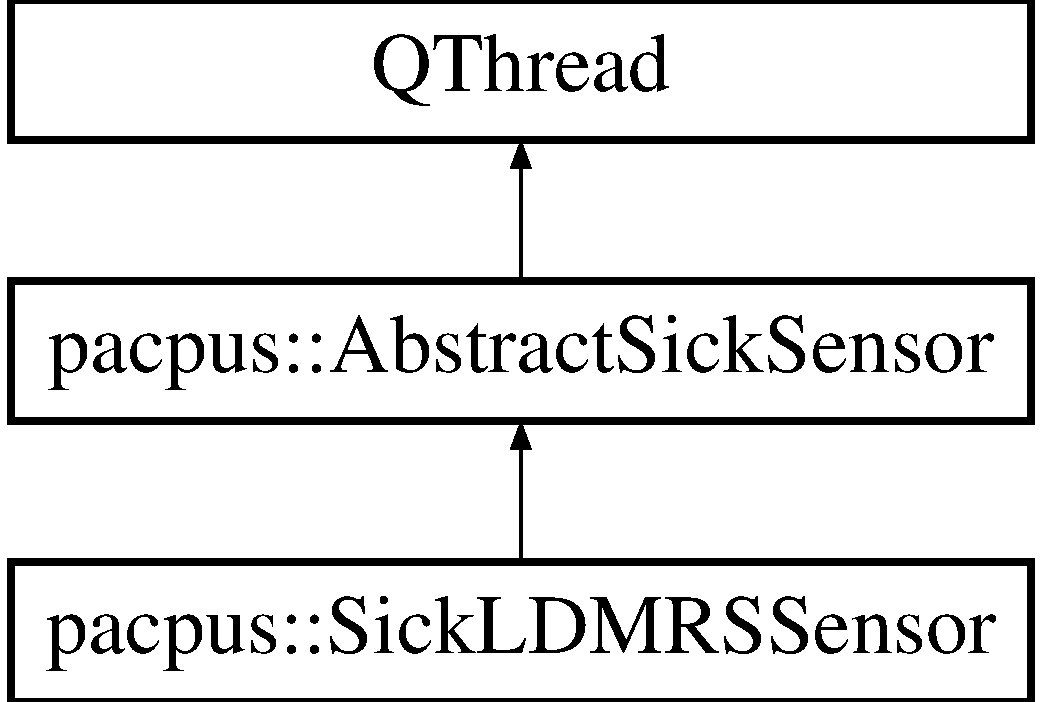
\includegraphics[height=3.000000cm]{classpacpus_1_1SickLDMRSSensor}
\end{center}
\end{figure}
\subsection*{Public Slots}
\begin{DoxyCompactItemize}
\item 
void \hyperlink{classpacpus_1_1SickLDMRSSensor_aff9f78d73af6aaf021cfbe9a521c6fad}{custom\-Event} (Q\-Event $\ast$e)
\begin{DoxyCompactList}\small\item\em custom\-Event allows to receive the incoming data and store them into known structures. \end{DoxyCompactList}\item 
\hypertarget{classpacpus_1_1SickLDMRSSensor_af88f26756d94460914ab88fb81f13768}{void \hyperlink{classpacpus_1_1SickLDMRSSensor_af88f26756d94460914ab88fb81f13768}{configure} ()}\label{classpacpus_1_1SickLDMRSSensor_af88f26756d94460914ab88fb81f13768}

\begin{DoxyCompactList}\small\item\em Configure the object, not used for the moment. \end{DoxyCompactList}\end{DoxyCompactItemize}
\subsection*{Public Member Functions}
\begin{DoxyCompactItemize}
\item 
\hypertarget{classpacpus_1_1SickLDMRSSensor_a0af00a3cf38fe5ae6a71038af4eb2a35}{\hyperlink{classpacpus_1_1SickLDMRSSensor_a0af00a3cf38fe5ae6a71038af4eb2a35}{Sick\-L\-D\-M\-R\-S\-Sensor} (Q\-Object $\ast$parent)}\label{classpacpus_1_1SickLDMRSSensor_a0af00a3cf38fe5ae6a71038af4eb2a35}

\begin{DoxyCompactList}\small\item\em Constructor. \end{DoxyCompactList}\item 
\hyperlink{classpacpus_1_1SickLDMRSSensor_a33518ebb2123cb2bccc68dfe1911769a}{Sick\-L\-D\-M\-R\-S\-Sensor} (Q\-Object $\ast$parent, Q\-String name, Q\-String ip, int port, int \hyperlink{classpacpus_1_1AbstractSickSensor_a2cefb63d92089cab86f874a3390acb28}{recording})
\begin{DoxyCompactList}\small\item\em \hyperlink{classpacpus_1_1SickLDMRSSensor}{Sick\-L\-D\-M\-R\-S\-Sensor} constructor. \end{DoxyCompactList}\item 
\hypertarget{classpacpus_1_1SickLDMRSSensor_af96ae9367377749421b5a541b107f83b}{\hyperlink{classpacpus_1_1SickLDMRSSensor_af96ae9367377749421b5a541b107f83b}{$\sim$\-Sick\-L\-D\-M\-R\-S\-Sensor} ()}\label{classpacpus_1_1SickLDMRSSensor_af96ae9367377749421b5a541b107f83b}

\begin{DoxyCompactList}\small\item\em Destructor. \end{DoxyCompactList}\item 
\hypertarget{classpacpus_1_1SickLDMRSSensor_a8579829420ffd7a6e9e85d2ae7adaea4}{void {\bfseries run} ()}\label{classpacpus_1_1SickLDMRSSensor_a8579829420ffd7a6e9e85d2ae7adaea4}

\item 
void \hyperlink{classpacpus_1_1SickLDMRSSensor_a5b3674df80e98093692fac9643819ab5}{stop\-Activity} ()
\item 
void \hyperlink{classpacpus_1_1SickLDMRSSensor_a2b82c6f677fe7e7e712b7397fb5390ee}{start\-Activity} ()
\item 
void \hyperlink{classpacpus_1_1SickLDMRSSensor_a5a3dd4f58b4d43fed06ff28db5822d5d}{split\-Packet} (const char $\ast$packet, const int length, road\-\_\-time\-\_\-t time)
\begin{DoxyCompactList}\small\item\em split\-Packet reconstitute incoming data and find messages. \end{DoxyCompactList}\item 
unsigned long \hyperlink{classpacpus_1_1SickLDMRSSensor_a01d9dc51e9220f828cb3651cf8b21e09}{process\-Message} (\hyperlink{classpacpus_1_1MessageLDMRS}{Message\-L\-D\-M\-R\-S} \&msg)
\begin{DoxyCompactList}\small\item\em Process/decode a message. \end{DoxyCompactList}\item 
u\-\_\-int32\-\_\-t \hyperlink{classpacpus_1_1SickLDMRSSensor_a223429320a452ab8bd50ec2b11691f91}{find\-Magic\-Word} (const char $\ast$message, const unsigned length)
\begin{DoxyCompactList}\small\item\em Find the position of the magic word into the array and returns this index. \end{DoxyCompactList}\item 
u\-\_\-int32\-\_\-t \hyperlink{classpacpus_1_1SickLDMRSSensor_ae128ee5ba4b2800822b9776a3001b999}{get\-Message\-Size} (const char $\ast$message, const unsigned length, const long magic\-Word\-Index)
\begin{DoxyCompactList}\small\item\em get\-Message\-Size get the message size of the entire message. \end{DoxyCompactList}\item 
bool \hyperlink{classpacpus_1_1SickLDMRSSensor_a1032c614191b0bbd9a5d2c36f362e70b}{is\-Message\-Complete} (const unsigned length, const long size)
\begin{DoxyCompactList}\small\item\em is\-Message\-Complete compare the size of the message read into the message and the length of the received data. \end{DoxyCompactList}\end{DoxyCompactItemize}
\subsection*{Public Attributes}
\begin{DoxyCompactItemize}
\item 
\hypertarget{classpacpus_1_1SickLDMRSSensor_a82b3667ed7a09898e73287d7ba620eb3}{\hyperlink{classpacpus_1_1SickSocket}{Sick\-Socket} $\ast$ \hyperlink{classpacpus_1_1SickLDMRSSensor_a82b3667ed7a09898e73287d7ba620eb3}{S\-\_\-socket}}\label{classpacpus_1_1SickLDMRSSensor_a82b3667ed7a09898e73287d7ba620eb3}

\begin{DoxyCompactList}\small\item\em S\-\_\-socket, used to receive and send data to the remote sensor. \end{DoxyCompactList}\end{DoxyCompactItemize}
\subsection*{Additional Inherited Members}


\subsection{Detailed Description}
The class implenting receiving, decoding and storing process of Sick L\-D-\/\-M\-R\-S data. 

This class can be used as a particular thread to acquire data from Sick L\-D\-M\-R\-S sensors. The Ethernet interface is used to get data from the sensor. Thus, the goal of this class is to get packets and decode them. Also, it offers the possibility to store all relevant information in two files (.dbt and .utc). It can be managed by \hyperlink{classpacpus_1_1SickComponent}{Sick\-Component} objects. 

\subsection{Constructor \& Destructor Documentation}
\hypertarget{classpacpus_1_1SickLDMRSSensor_a33518ebb2123cb2bccc68dfe1911769a}{\index{pacpus\-::\-Sick\-L\-D\-M\-R\-S\-Sensor@{pacpus\-::\-Sick\-L\-D\-M\-R\-S\-Sensor}!Sick\-L\-D\-M\-R\-S\-Sensor@{Sick\-L\-D\-M\-R\-S\-Sensor}}
\index{Sick\-L\-D\-M\-R\-S\-Sensor@{Sick\-L\-D\-M\-R\-S\-Sensor}!pacpus::SickLDMRSSensor@{pacpus\-::\-Sick\-L\-D\-M\-R\-S\-Sensor}}
\subsubsection[{Sick\-L\-D\-M\-R\-S\-Sensor}]{\setlength{\rightskip}{0pt plus 5cm}pacpus\-::\-Sick\-L\-D\-M\-R\-S\-Sensor\-::\-Sick\-L\-D\-M\-R\-S\-Sensor (
\begin{DoxyParamCaption}
\item[{Q\-Object $\ast$}]{parent, }
\item[{Q\-String}]{name, }
\item[{Q\-String}]{ip, }
\item[{int}]{port, }
\item[{int}]{recording}
\end{DoxyParamCaption}
)}}\label{classpacpus_1_1SickLDMRSSensor_a33518ebb2123cb2bccc68dfe1911769a}


\hyperlink{classpacpus_1_1SickLDMRSSensor}{Sick\-L\-D\-M\-R\-S\-Sensor} constructor. 


\begin{DoxyParams}{Parameters}
{\em parent} & Basically, a \hyperlink{classpacpus_1_1SickComponent}{Sick\-Component} object. \\
\hline
{\em name} & Name of the sensor in order to write on .dbt and .utc files and to recognize every sensors used. \\
\hline
{\em ip} & The I\-P address of the remote Sick L\-D\-M\-R\-S sensor. \\
\hline
{\em port} & The port of the remote Sick L\-D\-M\-R\-S sensor. \\
\hline
{\em recording} & If {\ttfamily true}, data is recorded into dbt + utc files. Data is not recorded otherwise. \\
\hline
\end{DoxyParams}


\subsection{Member Function Documentation}
\hypertarget{classpacpus_1_1SickLDMRSSensor_aff9f78d73af6aaf021cfbe9a521c6fad}{\index{pacpus\-::\-Sick\-L\-D\-M\-R\-S\-Sensor@{pacpus\-::\-Sick\-L\-D\-M\-R\-S\-Sensor}!custom\-Event@{custom\-Event}}
\index{custom\-Event@{custom\-Event}!pacpus::SickLDMRSSensor@{pacpus\-::\-Sick\-L\-D\-M\-R\-S\-Sensor}}
\subsubsection[{custom\-Event}]{\setlength{\rightskip}{0pt plus 5cm}void pacpus\-::\-Sick\-L\-D\-M\-R\-S\-Sensor\-::custom\-Event (
\begin{DoxyParamCaption}
\item[{Q\-Event $\ast$}]{e}
\end{DoxyParamCaption}
)\hspace{0.3cm}{\ttfamily [slot]}}}\label{classpacpus_1_1SickLDMRSSensor_aff9f78d73af6aaf021cfbe9a521c6fad}


custom\-Event allows to receive the incoming data and store them into known structures. 


\begin{DoxyParams}{Parameters}
{\em e} & Event that carries the Ethernet packets and receiving time. \\
\hline
\end{DoxyParams}
\hypertarget{classpacpus_1_1SickLDMRSSensor_a223429320a452ab8bd50ec2b11691f91}{\index{pacpus\-::\-Sick\-L\-D\-M\-R\-S\-Sensor@{pacpus\-::\-Sick\-L\-D\-M\-R\-S\-Sensor}!find\-Magic\-Word@{find\-Magic\-Word}}
\index{find\-Magic\-Word@{find\-Magic\-Word}!pacpus::SickLDMRSSensor@{pacpus\-::\-Sick\-L\-D\-M\-R\-S\-Sensor}}
\subsubsection[{find\-Magic\-Word}]{\setlength{\rightskip}{0pt plus 5cm}u\-\_\-int32\-\_\-t pacpus\-::\-Sick\-L\-D\-M\-R\-S\-Sensor\-::find\-Magic\-Word (
\begin{DoxyParamCaption}
\item[{const char $\ast$}]{message, }
\item[{const unsigned}]{length}
\end{DoxyParamCaption}
)}}\label{classpacpus_1_1SickLDMRSSensor_a223429320a452ab8bd50ec2b11691f91}


Find the position of the magic word into the array and returns this index. 


\begin{DoxyParams}{Parameters}
{\em message} & Array of characters, raw data received from sensor. \\
\hline
{\em length} & Length of the array. \\
\hline
\end{DoxyParams}
\begin{DoxyReturn}{Returns}

\begin{DoxyItemize}
\item {\bfseries -\/1} if no magic word is found
\item {\bfseries position} of the magic word otherwise 
\end{DoxyItemize}
\end{DoxyReturn}
\hypertarget{classpacpus_1_1SickLDMRSSensor_ae128ee5ba4b2800822b9776a3001b999}{\index{pacpus\-::\-Sick\-L\-D\-M\-R\-S\-Sensor@{pacpus\-::\-Sick\-L\-D\-M\-R\-S\-Sensor}!get\-Message\-Size@{get\-Message\-Size}}
\index{get\-Message\-Size@{get\-Message\-Size}!pacpus::SickLDMRSSensor@{pacpus\-::\-Sick\-L\-D\-M\-R\-S\-Sensor}}
\subsubsection[{get\-Message\-Size}]{\setlength{\rightskip}{0pt plus 5cm}u\-\_\-int32\-\_\-t pacpus\-::\-Sick\-L\-D\-M\-R\-S\-Sensor\-::get\-Message\-Size (
\begin{DoxyParamCaption}
\item[{const char $\ast$}]{message, }
\item[{const unsigned}]{length, }
\item[{const long}]{magic\-Word\-Index}
\end{DoxyParamCaption}
)}}\label{classpacpus_1_1SickLDMRSSensor_ae128ee5ba4b2800822b9776a3001b999}


get\-Message\-Size get the message size of the entire message. 


\begin{DoxyParams}{Parameters}
{\em message} & Raw data of the message. \\
\hline
{\em length} & Length of the raw data received. \\
\hline
{\em magic\-Word\-Index} & First element of the message, used to get the size of the message. \\
\hline
\end{DoxyParams}
\begin{DoxyReturn}{Returns}
The {\bfseries size} of the whole message.
\end{DoxyReturn}
The size of the message is found inside the message thanks to an offset after the index of the Magic Word.
\begin{DoxyItemize}
\item The first header of the message that contains the size of the message is in {\bfseries Big} {\bfseries Endian} format ! 
\end{DoxyItemize}\hypertarget{classpacpus_1_1SickLDMRSSensor_a1032c614191b0bbd9a5d2c36f362e70b}{\index{pacpus\-::\-Sick\-L\-D\-M\-R\-S\-Sensor@{pacpus\-::\-Sick\-L\-D\-M\-R\-S\-Sensor}!is\-Message\-Complete@{is\-Message\-Complete}}
\index{is\-Message\-Complete@{is\-Message\-Complete}!pacpus::SickLDMRSSensor@{pacpus\-::\-Sick\-L\-D\-M\-R\-S\-Sensor}}
\subsubsection[{is\-Message\-Complete}]{\setlength{\rightskip}{0pt plus 5cm}bool pacpus\-::\-Sick\-L\-D\-M\-R\-S\-Sensor\-::is\-Message\-Complete (
\begin{DoxyParamCaption}
\item[{const unsigned}]{length, }
\item[{const long}]{size}
\end{DoxyParamCaption}
)}}\label{classpacpus_1_1SickLDMRSSensor_a1032c614191b0bbd9a5d2c36f362e70b}


is\-Message\-Complete compare the size of the message read into the message and the length of the received data. 


\begin{DoxyParams}{Parameters}
{\em length} & Length of the received data. \\
\hline
{\em size} & Size of the message read. See get\-Message\-Size. \\
\hline
\end{DoxyParams}
\begin{DoxyReturn}{Returns}
{\bfseries true} if the message is complete, {\bfseries false} otherwise 
\end{DoxyReturn}
\hypertarget{classpacpus_1_1SickLDMRSSensor_a01d9dc51e9220f828cb3651cf8b21e09}{\index{pacpus\-::\-Sick\-L\-D\-M\-R\-S\-Sensor@{pacpus\-::\-Sick\-L\-D\-M\-R\-S\-Sensor}!process\-Message@{process\-Message}}
\index{process\-Message@{process\-Message}!pacpus::SickLDMRSSensor@{pacpus\-::\-Sick\-L\-D\-M\-R\-S\-Sensor}}
\subsubsection[{process\-Message}]{\setlength{\rightskip}{0pt plus 5cm}unsigned long pacpus\-::\-Sick\-L\-D\-M\-R\-S\-Sensor\-::process\-Message (
\begin{DoxyParamCaption}
\item[{{\bf Message\-L\-D\-M\-R\-S} \&}]{msg}
\end{DoxyParamCaption}
)}}\label{classpacpus_1_1SickLDMRSSensor_a01d9dc51e9220f828cb3651cf8b21e09}


Process/decode a message. 


\begin{DoxyParams}{Parameters}
{\em msg} & The message is encapsulated into a \hyperlink{classpacpus_1_1MessageLDMRS}{Message\-L\-D\-M\-R\-S} \\
\hline
\end{DoxyParams}
\begin{DoxyReturn}{Returns}
Type of the message
\end{DoxyReturn}
Process the raw data of the message and update the \hyperlink{classpacpus_1_1MessageLDMRS}{Message\-L\-D\-M\-R\-S} object passed \-: it fills the 2 headers (message and scan) and replace the body field of the Message\-L\-D\-R\-M\-S object by an array of \hyperlink{structpacpus_1_1ScanPoint}{Scan\-Point}.
\begin{DoxyItemize}
\item {\bfseries Warning} \-: the process of object data type is not implemented yet ! 
\end{DoxyItemize}\hypertarget{classpacpus_1_1SickLDMRSSensor_a5a3dd4f58b4d43fed06ff28db5822d5d}{\index{pacpus\-::\-Sick\-L\-D\-M\-R\-S\-Sensor@{pacpus\-::\-Sick\-L\-D\-M\-R\-S\-Sensor}!split\-Packet@{split\-Packet}}
\index{split\-Packet@{split\-Packet}!pacpus::SickLDMRSSensor@{pacpus\-::\-Sick\-L\-D\-M\-R\-S\-Sensor}}
\subsubsection[{split\-Packet}]{\setlength{\rightskip}{0pt plus 5cm}void pacpus\-::\-Sick\-L\-D\-M\-R\-S\-Sensor\-::split\-Packet (
\begin{DoxyParamCaption}
\item[{const char $\ast$}]{packet, }
\item[{const int}]{length, }
\item[{road\-\_\-time\-\_\-t}]{time}
\end{DoxyParamCaption}
)}}\label{classpacpus_1_1SickLDMRSSensor_a5a3dd4f58b4d43fed06ff28db5822d5d}


split\-Packet reconstitute incoming data and find messages. 


\begin{DoxyParams}{Parameters}
{\em packet} & Raw data coming from the sensor. \\
\hline
{\em length} & Length of the data. \\
\hline
{\em time} & Time of the last received data.\\
\hline
\end{DoxyParams}
Analyse the ethernet packet received from the Sick sensor and try to find a complete message (scan data message or object message) If a message has been found it is added at the end of the message list else the pending bytes are stored to be analyzed by further incoming data. \hypertarget{classpacpus_1_1SickLDMRSSensor_a2b82c6f677fe7e7e712b7397fb5390ee}{\index{pacpus\-::\-Sick\-L\-D\-M\-R\-S\-Sensor@{pacpus\-::\-Sick\-L\-D\-M\-R\-S\-Sensor}!start\-Activity@{start\-Activity}}
\index{start\-Activity@{start\-Activity}!pacpus::SickLDMRSSensor@{pacpus\-::\-Sick\-L\-D\-M\-R\-S\-Sensor}}
\subsubsection[{start\-Activity}]{\setlength{\rightskip}{0pt plus 5cm}void pacpus\-::\-Sick\-L\-D\-M\-R\-S\-Sensor\-::start\-Activity (
\begin{DoxyParamCaption}
{}
\end{DoxyParamCaption}
)\hspace{0.3cm}{\ttfamily [virtual]}}}\label{classpacpus_1_1SickLDMRSSensor_a2b82c6f677fe7e7e712b7397fb5390ee}
To start the processing thread 

Implements \hyperlink{classpacpus_1_1AbstractSickSensor_af8e017866cf70db766dbd11b60a52425}{pacpus\-::\-Abstract\-Sick\-Sensor}.

\hypertarget{classpacpus_1_1SickLDMRSSensor_a5b3674df80e98093692fac9643819ab5}{\index{pacpus\-::\-Sick\-L\-D\-M\-R\-S\-Sensor@{pacpus\-::\-Sick\-L\-D\-M\-R\-S\-Sensor}!stop\-Activity@{stop\-Activity}}
\index{stop\-Activity@{stop\-Activity}!pacpus::SickLDMRSSensor@{pacpus\-::\-Sick\-L\-D\-M\-R\-S\-Sensor}}
\subsubsection[{stop\-Activity}]{\setlength{\rightskip}{0pt plus 5cm}void pacpus\-::\-Sick\-L\-D\-M\-R\-S\-Sensor\-::stop\-Activity (
\begin{DoxyParamCaption}
{}
\end{DoxyParamCaption}
)\hspace{0.3cm}{\ttfamily [virtual]}}}\label{classpacpus_1_1SickLDMRSSensor_a5b3674df80e98093692fac9643819ab5}
To stop the processing thread 

Implements \hyperlink{classpacpus_1_1AbstractSickSensor_a14c6da8df61d91f2b63439df00fd5d6a}{pacpus\-::\-Abstract\-Sick\-Sensor}.



The documentation for this class was generated from the following files\-:\begin{DoxyCompactItemize}
\item 
Sick\-L\-D\-M\-R\-S\-Sensor.\-h\item 
Sick\-L\-D\-M\-R\-S\-Sensor.\-cpp\end{DoxyCompactItemize}

\hypertarget{structpacpus_1_1SickLMS__dbt}{\section{pacpus\-:\-:Sick\-L\-M\-S\-\_\-dbt Struct Reference}
\label{structpacpus_1_1SickLMS__dbt}\index{pacpus\-::\-Sick\-L\-M\-S\-\_\-dbt@{pacpus\-::\-Sick\-L\-M\-S\-\_\-dbt}}
}
\subsection*{Public Attributes}
\begin{DoxyCompactItemize}
\item 
\hypertarget{structpacpus_1_1SickLMS__dbt_a43c6abf5a37f9432442e25c95e375e90}{u\-\_\-int16\-\_\-t \hyperlink{structpacpus_1_1SickLMS__dbt_a43c6abf5a37f9432442e25c95e375e90}{scan\-Number}}\label{structpacpus_1_1SickLMS__dbt_a43c6abf5a37f9432442e25c95e375e90}

\begin{DoxyCompactList}\small\item\em number of the scan \end{DoxyCompactList}\item 
u\-\_\-int16\-\_\-t \hyperlink{structpacpus_1_1SickLMS__dbt_a10e25b3d9019c08a41ea8f52fc323345}{scanner\-Status}
\item 
\hypertarget{structpacpus_1_1SickLMS__dbt_a46f6d62185441de61f75581c19efa7a3}{road\-\_\-time\-\_\-t \hyperlink{structpacpus_1_1SickLMS__dbt_a46f6d62185441de61f75581c19efa7a3}{time}}\label{structpacpus_1_1SickLMS__dbt_a46f6d62185441de61f75581c19efa7a3}

\begin{DoxyCompactList}\small\item\em D\-B\-T timestamp. \end{DoxyCompactList}\item 
\hypertarget{structpacpus_1_1SickLMS__dbt_a5fc03bad1484c48a8dafb98d7d3b4f52}{road\-\_\-timerange\-\_\-t \hyperlink{structpacpus_1_1SickLMS__dbt_a5fc03bad1484c48a8dafb98d7d3b4f52}{timerange}}\label{structpacpus_1_1SickLMS__dbt_a5fc03bad1484c48a8dafb98d7d3b4f52}

\begin{DoxyCompactList}\small\item\em D\-B\-T timerange. \end{DoxyCompactList}\item 
\hypertarget{structpacpus_1_1SickLMS__dbt_a578213dd3cc30c4990911398d52cb8cf}{u\-\_\-int32\-\_\-t \hyperlink{structpacpus_1_1SickLMS__dbt_a578213dd3cc30c4990911398d52cb8cf}{scan\-Frequency}}\label{structpacpus_1_1SickLMS__dbt_a578213dd3cc30c4990911398d52cb8cf}

\begin{DoxyCompactList}\small\item\em Frequency of the scan \mbox{[}1/100 Hz\mbox{]}. \end{DoxyCompactList}\item 
\hypertarget{structpacpus_1_1SickLMS__dbt_acbc0527837e1a0442420c0d79aa4f72f}{u\-\_\-int32\-\_\-t \hyperlink{structpacpus_1_1SickLMS__dbt_acbc0527837e1a0442420c0d79aa4f72f}{angle\-Resolution}}\label{structpacpus_1_1SickLMS__dbt_acbc0527837e1a0442420c0d79aa4f72f}

\begin{DoxyCompactList}\small\item\em Angle resolution (default is 5000 $<$=$>$ 0.\-5 degree) \mbox{[}1/10000 degree\mbox{]}. \end{DoxyCompactList}\item 
\hypertarget{structpacpus_1_1SickLMS__dbt_a11ac14e5c8662c054f750ded3cb6da71}{int32\-\_\-t \hyperlink{structpacpus_1_1SickLMS__dbt_a11ac14e5c8662c054f750ded3cb6da71}{start\-Angle}}\label{structpacpus_1_1SickLMS__dbt_a11ac14e5c8662c054f750ded3cb6da71}

\begin{DoxyCompactList}\small\item\em Angle of the first scanned point. \end{DoxyCompactList}\item 
\hypertarget{structpacpus_1_1SickLMS__dbt_a2b8b48872c09823f22f98f1085a065a3}{int \hyperlink{structpacpus_1_1SickLMS__dbt_a2b8b48872c09823f22f98f1085a065a3}{dist\-\_\-len1}}\label{structpacpus_1_1SickLMS__dbt_a2b8b48872c09823f22f98f1085a065a3}

\begin{DoxyCompactList}\small\item\em Number of points (1st echo). \end{DoxyCompactList}\item 
\hypertarget{structpacpus_1_1SickLMS__dbt_ac963dda9a0489f79288c972419d94541}{uint32\-\_\-t \hyperlink{structpacpus_1_1SickLMS__dbt_ac963dda9a0489f79288c972419d94541}{data\-Pos\-\_\-dist1}}\label{structpacpus_1_1SickLMS__dbt_ac963dda9a0489f79288c972419d94541}

\begin{DoxyCompactList}\small\item\em Distance between the sensor and the remote point (1st echo). \end{DoxyCompactList}\item 
\hypertarget{structpacpus_1_1SickLMS__dbt_afb7fcb7cc7ec15ad7c0ce63978109adb}{int \hyperlink{structpacpus_1_1SickLMS__dbt_afb7fcb7cc7ec15ad7c0ce63978109adb}{dist\-\_\-len2}}\label{structpacpus_1_1SickLMS__dbt_afb7fcb7cc7ec15ad7c0ce63978109adb}

\begin{DoxyCompactList}\small\item\em Number of points (2nd echo). \end{DoxyCompactList}\item 
\hypertarget{structpacpus_1_1SickLMS__dbt_a405a50a42f60b5f3452b45433ee397f4}{uint32\-\_\-t \hyperlink{structpacpus_1_1SickLMS__dbt_a405a50a42f60b5f3452b45433ee397f4}{data\-Pos\-\_\-dist2}}\label{structpacpus_1_1SickLMS__dbt_a405a50a42f60b5f3452b45433ee397f4}

\begin{DoxyCompactList}\small\item\em Distance between the sensor and the remote point (2nd echo). \end{DoxyCompactList}\item 
\hypertarget{structpacpus_1_1SickLMS__dbt_aa457a25a6b3511055bbdbc34a1a9f5e2}{int \hyperlink{structpacpus_1_1SickLMS__dbt_aa457a25a6b3511055bbdbc34a1a9f5e2}{dist\-\_\-len3}}\label{structpacpus_1_1SickLMS__dbt_aa457a25a6b3511055bbdbc34a1a9f5e2}

\begin{DoxyCompactList}\small\item\em Number of points (3rd echo). \end{DoxyCompactList}\item 
\hypertarget{structpacpus_1_1SickLMS__dbt_afaea29ff718ae370c1ddc03170bf2d58}{uint32\-\_\-t \hyperlink{structpacpus_1_1SickLMS__dbt_afaea29ff718ae370c1ddc03170bf2d58}{data\-Pos\-\_\-dist3}}\label{structpacpus_1_1SickLMS__dbt_afaea29ff718ae370c1ddc03170bf2d58}

\begin{DoxyCompactList}\small\item\em Distance between the sensor and the remote point (3rd echo). {\bfseries L\-M\-S5xx} {\bfseries only}. \end{DoxyCompactList}\item 
\hypertarget{structpacpus_1_1SickLMS__dbt_a2c9ed5c2a00dd9f367011da96135a7d3}{int \hyperlink{structpacpus_1_1SickLMS__dbt_a2c9ed5c2a00dd9f367011da96135a7d3}{dist\-\_\-len4}}\label{structpacpus_1_1SickLMS__dbt_a2c9ed5c2a00dd9f367011da96135a7d3}

\begin{DoxyCompactList}\small\item\em Number of points (4th echo). \end{DoxyCompactList}\item 
\hypertarget{structpacpus_1_1SickLMS__dbt_a5ead9c1691285121f3f5dc4c9678779e}{uint32\-\_\-t \hyperlink{structpacpus_1_1SickLMS__dbt_a5ead9c1691285121f3f5dc4c9678779e}{data\-Pos\-\_\-dist4}}\label{structpacpus_1_1SickLMS__dbt_a5ead9c1691285121f3f5dc4c9678779e}

\begin{DoxyCompactList}\small\item\em Distance between the sensor and the remote point (4th echo). {\bfseries L\-M\-S5xx} {\bfseries only}. \end{DoxyCompactList}\item 
\hypertarget{structpacpus_1_1SickLMS__dbt_a3e57b76ae42d4ef76b065f6caf09d3ba}{int \hyperlink{structpacpus_1_1SickLMS__dbt_a3e57b76ae42d4ef76b065f6caf09d3ba}{dist\-\_\-len5}}\label{structpacpus_1_1SickLMS__dbt_a3e57b76ae42d4ef76b065f6caf09d3ba}

\begin{DoxyCompactList}\small\item\em Number of points (5th echo). \end{DoxyCompactList}\item 
\hypertarget{structpacpus_1_1SickLMS__dbt_ad46c09e76ba9eb92dba67aaa52d42322}{uint32\-\_\-t \hyperlink{structpacpus_1_1SickLMS__dbt_ad46c09e76ba9eb92dba67aaa52d42322}{data\-Pos\-\_\-dist5}}\label{structpacpus_1_1SickLMS__dbt_ad46c09e76ba9eb92dba67aaa52d42322}

\begin{DoxyCompactList}\small\item\em Distance between the sensor and the remote point (5th echo). {\bfseries L\-M\-S5xx} {\bfseries only}. \end{DoxyCompactList}\item 
\hypertarget{structpacpus_1_1SickLMS__dbt_a28db8f5f2eb2b3f7674fed018d68a753}{int \hyperlink{structpacpus_1_1SickLMS__dbt_a28db8f5f2eb2b3f7674fed018d68a753}{rssi\-\_\-len1}}\label{structpacpus_1_1SickLMS__dbt_a28db8f5f2eb2b3f7674fed018d68a753}

\begin{DoxyCompactList}\small\item\em Number of energy values (1st echo). \end{DoxyCompactList}\item 
\hypertarget{structpacpus_1_1SickLMS__dbt_a944d22badb118ea88ce24e308e25b50d}{uint32\-\_\-t \hyperlink{structpacpus_1_1SickLMS__dbt_a944d22badb118ea88ce24e308e25b50d}{data\-Pos\-\_\-rssi1}}\label{structpacpus_1_1SickLMS__dbt_a944d22badb118ea88ce24e308e25b50d}

\begin{DoxyCompactList}\small\item\em Energy of the returned pulse (1st echo). {\bfseries L\-M\-S1xx} {\bfseries only}. \end{DoxyCompactList}\item 
\hypertarget{structpacpus_1_1SickLMS__dbt_a99fb6cb7c53cb0115a82e7414a60ffcd}{int \hyperlink{structpacpus_1_1SickLMS__dbt_a99fb6cb7c53cb0115a82e7414a60ffcd}{rssi\-\_\-len2}}\label{structpacpus_1_1SickLMS__dbt_a99fb6cb7c53cb0115a82e7414a60ffcd}

\begin{DoxyCompactList}\small\item\em Number of energy values (2nd echo). \end{DoxyCompactList}\item 
\hypertarget{structpacpus_1_1SickLMS__dbt_a4a1509ac1b9821bb55d42c9fd1e25d12}{uint32\-\_\-t \hyperlink{structpacpus_1_1SickLMS__dbt_a4a1509ac1b9821bb55d42c9fd1e25d12}{data\-Pos\-\_\-rssi2}}\label{structpacpus_1_1SickLMS__dbt_a4a1509ac1b9821bb55d42c9fd1e25d12}

\begin{DoxyCompactList}\small\item\em Energy of the returned pulse (2nd echo). {\bfseries L\-M\-S1xx} {\bfseries only}. \end{DoxyCompactList}\end{DoxyCompactItemize}


\subsection{Member Data Documentation}
\hypertarget{structpacpus_1_1SickLMS__dbt_a10e25b3d9019c08a41ea8f52fc323345}{\index{pacpus\-::\-Sick\-L\-M\-S\-\_\-dbt@{pacpus\-::\-Sick\-L\-M\-S\-\_\-dbt}!scanner\-Status@{scanner\-Status}}
\index{scanner\-Status@{scanner\-Status}!pacpus::SickLMS_dbt@{pacpus\-::\-Sick\-L\-M\-S\-\_\-dbt}}
\subsubsection[{scanner\-Status}]{\setlength{\rightskip}{0pt plus 5cm}u\-\_\-int16\-\_\-t pacpus\-::\-Sick\-L\-M\-S\-\_\-dbt\-::scanner\-Status}}\label{structpacpus_1_1SickLMS__dbt_a10e25b3d9019c08a41ea8f52fc323345}

\begin{DoxyItemize}
\item 00 00 O\-K
\item 00 01 Error
\item 00 02 Pollution Warning
\item 00 04 Pollution Error 
\end{DoxyItemize}

The documentation for this struct was generated from the following file\-:\begin{DoxyCompactItemize}
\item 
Sick\-L\-M\-S\-Data.\-h\end{DoxyCompactItemize}

\hypertarget{classpacpus_1_1SickLMSSensor}{\section{pacpus\-:\-:Sick\-L\-M\-S\-Sensor Class Reference}
\label{classpacpus_1_1SickLMSSensor}\index{pacpus\-::\-Sick\-L\-M\-S\-Sensor@{pacpus\-::\-Sick\-L\-M\-S\-Sensor}}
}


The class implenting receiving, decoding and storing process of Sick L\-M\-S data.  




{\ttfamily \#include $<$Sick\-L\-M\-S\-Sensor.\-h$>$}

Inheritance diagram for pacpus\-:\-:Sick\-L\-M\-S\-Sensor\-:\begin{figure}[H]
\begin{center}
\leavevmode
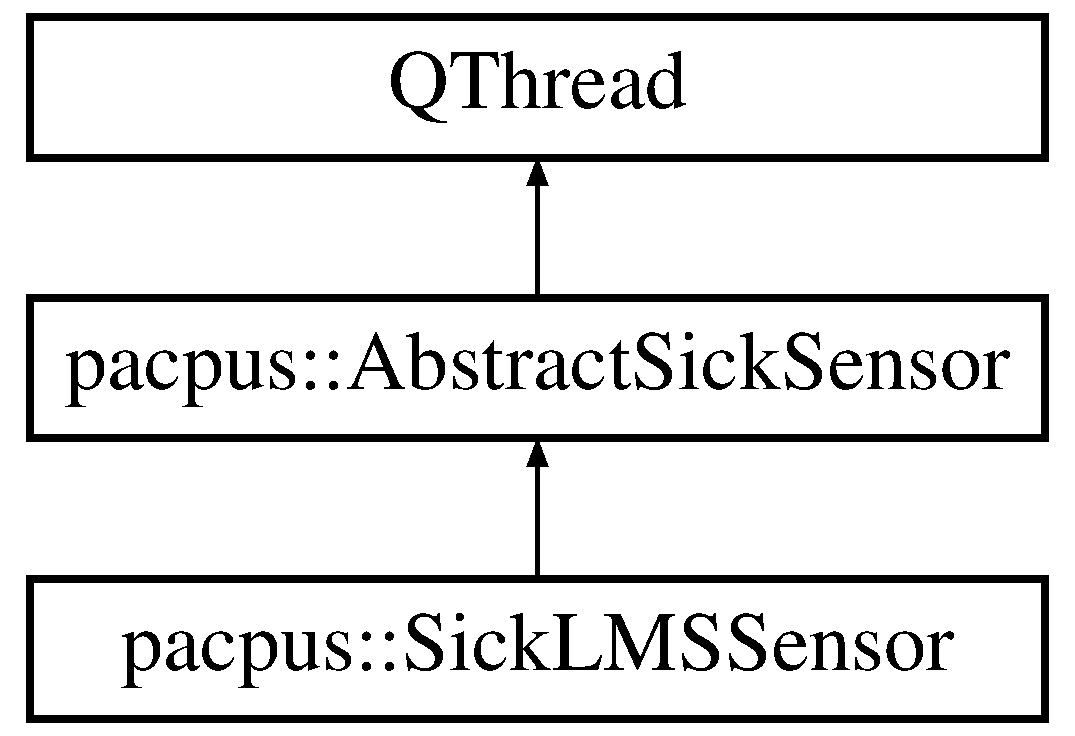
\includegraphics[height=3.000000cm]{classpacpus_1_1SickLMSSensor}
\end{center}
\end{figure}
\subsection*{Public Slots}
\begin{DoxyCompactItemize}
\item 
void \hyperlink{classpacpus_1_1SickLMSSensor_a1ec604914c64ed7d5d884ae55472499f}{custom\-Event} (Q\-Event $\ast$e)
\begin{DoxyCompactList}\small\item\em custom\-Event allows to receive the incoming data and store them into known structures. \end{DoxyCompactList}\item 
\hypertarget{classpacpus_1_1SickLMSSensor_a31986523670fd4ca7173a30bc40688b4}{void \hyperlink{classpacpus_1_1SickLMSSensor_a31986523670fd4ca7173a30bc40688b4}{configure} ()}\label{classpacpus_1_1SickLMSSensor_a31986523670fd4ca7173a30bc40688b4}

\begin{DoxyCompactList}\small\item\em Configure the object, not used for the moment. \end{DoxyCompactList}\end{DoxyCompactItemize}
\subsection*{Public Member Functions}
\begin{DoxyCompactItemize}
\item 
\hypertarget{classpacpus_1_1SickLMSSensor_a9e87f9cb5fd8c978af8d2633d98c0405}{\hyperlink{classpacpus_1_1SickLMSSensor_a9e87f9cb5fd8c978af8d2633d98c0405}{Sick\-L\-M\-S\-Sensor} (Q\-Object $\ast$parent)}\label{classpacpus_1_1SickLMSSensor_a9e87f9cb5fd8c978af8d2633d98c0405}

\begin{DoxyCompactList}\small\item\em Constructor. \end{DoxyCompactList}\item 
\hyperlink{classpacpus_1_1SickLMSSensor_ad1e27ae5fb0421011f3f6bf464f7e42c}{Sick\-L\-M\-S\-Sensor} (Q\-Object $\ast$parent, Q\-String name, Q\-String ip, int port, int \hyperlink{classpacpus_1_1AbstractSickSensor_a2cefb63d92089cab86f874a3390acb28}{recording})
\begin{DoxyCompactList}\small\item\em \hyperlink{classpacpus_1_1SickLMSSensor}{Sick\-L\-M\-S\-Sensor} constructor. \end{DoxyCompactList}\item 
\hypertarget{classpacpus_1_1SickLMSSensor_a557fadfe7ac1a08f9d2ee2d88cc66a61}{\hyperlink{classpacpus_1_1SickLMSSensor_a557fadfe7ac1a08f9d2ee2d88cc66a61}{$\sim$\-Sick\-L\-M\-S\-Sensor} ()}\label{classpacpus_1_1SickLMSSensor_a557fadfe7ac1a08f9d2ee2d88cc66a61}

\begin{DoxyCompactList}\small\item\em Destructor. \end{DoxyCompactList}\item 
\hypertarget{classpacpus_1_1SickLMSSensor_ab598fdcee13cb01624dfd806e524afac}{void {\bfseries run} ()}\label{classpacpus_1_1SickLMSSensor_ab598fdcee13cb01624dfd806e524afac}

\item 
void \hyperlink{classpacpus_1_1SickLMSSensor_a082417a753cef1d4f726c50b2e14a4d0}{stop\-Activity} ()
\item 
void \hyperlink{classpacpus_1_1SickLMSSensor_a6268a9b5b17db84b662c562ea332541f}{start\-Activity} ()
\item 
void \hyperlink{classpacpus_1_1SickLMSSensor_a3182c21683131e52c520d45bd4a23dae}{reconstitute\-Message} (const char $\ast$packet, const int length, road\-\_\-time\-\_\-t time)
\begin{DoxyCompactList}\small\item\em reconstitute\-Message reconstitute a complete message from received packets \end{DoxyCompactList}\item 
int \hyperlink{classpacpus_1_1SickLMSSensor_a4ba9228b2f513fc3d7dcac5813065212}{process\-Scan\-Data} (\hyperlink{classpacpus_1_1MessageLMS}{Message\-L\-M\-S} $\ast$msg)
\begin{DoxyCompactList}\small\item\em process\-Scan\-Data Parse information and process every needed values. \end{DoxyCompactList}\item 
int \hyperlink{classpacpus_1_1SickLMSSensor_a0993b71ac52777e6588e57bb261c8ae9}{is\-Message\-Complete} (const char $\ast$packets, unsigned int size)
\begin{DoxyCompactList}\small\item\em is\-Message\-Complete find the $<$\-E\-T\-X$>$ character (corresponding to the end of a message). \end{DoxyCompactList}\end{DoxyCompactItemize}
\subsection*{Public Attributes}
\begin{DoxyCompactItemize}
\item 
\hypertarget{classpacpus_1_1SickLMSSensor_a33a0af999049a7d9a35e1719d9d9cd48}{\hyperlink{classpacpus_1_1SickSocket}{Sick\-Socket} $\ast$ \hyperlink{classpacpus_1_1SickLMSSensor_a33a0af999049a7d9a35e1719d9d9cd48}{S\-\_\-socket}}\label{classpacpus_1_1SickLMSSensor_a33a0af999049a7d9a35e1719d9d9cd48}

\begin{DoxyCompactList}\small\item\em S\-\_\-socket, used to receive and send data to the remote sensor. \end{DoxyCompactList}\end{DoxyCompactItemize}
\subsection*{Additional Inherited Members}


\subsection{Detailed Description}
The class implenting receiving, decoding and storing process of Sick L\-M\-S data. 

This class can be used as a particular thread to acquire data from Sick L\-D\-M\-R\-S sensors. The Ethernet interface is used to get data from the sensor. Thus, the goal of this class is to get packets and decode them. Also, it offers the possibility to store all relevant information in two files (.dbt and .utc). It can be managed by \hyperlink{classpacpus_1_1SickComponent}{Sick\-Component} objects. 

\subsection{Constructor \& Destructor Documentation}
\hypertarget{classpacpus_1_1SickLMSSensor_ad1e27ae5fb0421011f3f6bf464f7e42c}{\index{pacpus\-::\-Sick\-L\-M\-S\-Sensor@{pacpus\-::\-Sick\-L\-M\-S\-Sensor}!Sick\-L\-M\-S\-Sensor@{Sick\-L\-M\-S\-Sensor}}
\index{Sick\-L\-M\-S\-Sensor@{Sick\-L\-M\-S\-Sensor}!pacpus::SickLMSSensor@{pacpus\-::\-Sick\-L\-M\-S\-Sensor}}
\subsubsection[{Sick\-L\-M\-S\-Sensor}]{\setlength{\rightskip}{0pt plus 5cm}pacpus\-::\-Sick\-L\-M\-S\-Sensor\-::\-Sick\-L\-M\-S\-Sensor (
\begin{DoxyParamCaption}
\item[{Q\-Object $\ast$}]{parent, }
\item[{Q\-String}]{name, }
\item[{Q\-String}]{ip, }
\item[{int}]{port, }
\item[{int}]{recording}
\end{DoxyParamCaption}
)}}\label{classpacpus_1_1SickLMSSensor_ad1e27ae5fb0421011f3f6bf464f7e42c}


\hyperlink{classpacpus_1_1SickLMSSensor}{Sick\-L\-M\-S\-Sensor} constructor. 


\begin{DoxyParams}{Parameters}
{\em parent} & Basically, a \hyperlink{classpacpus_1_1SickComponent}{Sick\-Component} object. \\
\hline
{\em name} & Name of the sensor in order to write on .dbt and .utc files and to recognize every sensors used. \\
\hline
{\em ip} & The I\-P address of the remote Sick L\-M\-S sensor. \\
\hline
{\em port} & The port of the remote Sick L\-M\-S sensor. \\
\hline
{\em recording} & If {\ttfamily true}, data is recorded into dbt + utc files. Data is not recorded otherwise. \\
\hline
\end{DoxyParams}


\subsection{Member Function Documentation}
\hypertarget{classpacpus_1_1SickLMSSensor_a1ec604914c64ed7d5d884ae55472499f}{\index{pacpus\-::\-Sick\-L\-M\-S\-Sensor@{pacpus\-::\-Sick\-L\-M\-S\-Sensor}!custom\-Event@{custom\-Event}}
\index{custom\-Event@{custom\-Event}!pacpus::SickLMSSensor@{pacpus\-::\-Sick\-L\-M\-S\-Sensor}}
\subsubsection[{custom\-Event}]{\setlength{\rightskip}{0pt plus 5cm}void pacpus\-::\-Sick\-L\-M\-S\-Sensor\-::custom\-Event (
\begin{DoxyParamCaption}
\item[{Q\-Event $\ast$}]{e}
\end{DoxyParamCaption}
)\hspace{0.3cm}{\ttfamily [slot]}}}\label{classpacpus_1_1SickLMSSensor_a1ec604914c64ed7d5d884ae55472499f}


custom\-Event allows to receive the incoming data and store them into known structures. 


\begin{DoxyParams}{Parameters}
{\em e} & Event that carries the Ethernet packets and receiving time. \\
\hline
\end{DoxyParams}
\hypertarget{classpacpus_1_1SickLMSSensor_a0993b71ac52777e6588e57bb261c8ae9}{\index{pacpus\-::\-Sick\-L\-M\-S\-Sensor@{pacpus\-::\-Sick\-L\-M\-S\-Sensor}!is\-Message\-Complete@{is\-Message\-Complete}}
\index{is\-Message\-Complete@{is\-Message\-Complete}!pacpus::SickLMSSensor@{pacpus\-::\-Sick\-L\-M\-S\-Sensor}}
\subsubsection[{is\-Message\-Complete}]{\setlength{\rightskip}{0pt plus 5cm}int pacpus\-::\-Sick\-L\-M\-S\-Sensor\-::is\-Message\-Complete (
\begin{DoxyParamCaption}
\item[{const char $\ast$}]{packets, }
\item[{unsigned int}]{size}
\end{DoxyParamCaption}
)}}\label{classpacpus_1_1SickLMSSensor_a0993b71ac52777e6588e57bb261c8ae9}


is\-Message\-Complete find the $<$\-E\-T\-X$>$ character (corresponding to the end of a message). 


\begin{DoxyParams}{Parameters}
{\em packets} & Raw data. \\
\hline
{\em size} & Size of raw data. \\
\hline
\end{DoxyParams}
\begin{DoxyReturn}{Returns}
The index of the $<$\-E\-T\-X$>$ character. 
\end{DoxyReturn}
\hypertarget{classpacpus_1_1SickLMSSensor_a4ba9228b2f513fc3d7dcac5813065212}{\index{pacpus\-::\-Sick\-L\-M\-S\-Sensor@{pacpus\-::\-Sick\-L\-M\-S\-Sensor}!process\-Scan\-Data@{process\-Scan\-Data}}
\index{process\-Scan\-Data@{process\-Scan\-Data}!pacpus::SickLMSSensor@{pacpus\-::\-Sick\-L\-M\-S\-Sensor}}
\subsubsection[{process\-Scan\-Data}]{\setlength{\rightskip}{0pt plus 5cm}int pacpus\-::\-Sick\-L\-M\-S\-Sensor\-::process\-Scan\-Data (
\begin{DoxyParamCaption}
\item[{{\bf Message\-L\-M\-S} $\ast$}]{msg}
\end{DoxyParamCaption}
)}}\label{classpacpus_1_1SickLMSSensor_a4ba9228b2f513fc3d7dcac5813065212}


process\-Scan\-Data Parse information and process every needed values. 


\begin{DoxyParams}{Parameters}
{\em msg} & Carries a message. split\-Message field of \hyperlink{classpacpus_1_1MessageLMS}{Message\-L\-M\-S} must be filled. \\
\hline
\end{DoxyParams}
\begin{DoxyReturn}{Returns}
Not used for the moment. 
\end{DoxyReturn}
\hypertarget{classpacpus_1_1SickLMSSensor_a3182c21683131e52c520d45bd4a23dae}{\index{pacpus\-::\-Sick\-L\-M\-S\-Sensor@{pacpus\-::\-Sick\-L\-M\-S\-Sensor}!reconstitute\-Message@{reconstitute\-Message}}
\index{reconstitute\-Message@{reconstitute\-Message}!pacpus::SickLMSSensor@{pacpus\-::\-Sick\-L\-M\-S\-Sensor}}
\subsubsection[{reconstitute\-Message}]{\setlength{\rightskip}{0pt plus 5cm}void pacpus\-::\-Sick\-L\-M\-S\-Sensor\-::reconstitute\-Message (
\begin{DoxyParamCaption}
\item[{const char $\ast$}]{packet, }
\item[{const int}]{length, }
\item[{road\-\_\-time\-\_\-t}]{time}
\end{DoxyParamCaption}
)}}\label{classpacpus_1_1SickLMSSensor_a3182c21683131e52c520d45bd4a23dae}


reconstitute\-Message reconstitute a complete message from received packets 


\begin{DoxyParams}{Parameters}
{\em packet} & Raw data coming from the sensor. \\
\hline
{\em length} & Length of the raw data received. \\
\hline
{\em time} & Time of the last received data.\\
\hline
\end{DoxyParams}
A message starts with a $<$\-S\-T\-X$>$ (0x02 in A\-S\-C\-I\-I) char and ends with $<$\-E\-T\-X$>$ (0x03 in A\-S\-C\-I\-I). This function stores packets until a complete message is received. In this case, the message is added to the list of \hyperlink{classpacpus_1_1MessageLMS}{Message\-L\-M\-S}, msg\-List. \hypertarget{classpacpus_1_1SickLMSSensor_a6268a9b5b17db84b662c562ea332541f}{\index{pacpus\-::\-Sick\-L\-M\-S\-Sensor@{pacpus\-::\-Sick\-L\-M\-S\-Sensor}!start\-Activity@{start\-Activity}}
\index{start\-Activity@{start\-Activity}!pacpus::SickLMSSensor@{pacpus\-::\-Sick\-L\-M\-S\-Sensor}}
\subsubsection[{start\-Activity}]{\setlength{\rightskip}{0pt plus 5cm}void pacpus\-::\-Sick\-L\-M\-S\-Sensor\-::start\-Activity (
\begin{DoxyParamCaption}
{}
\end{DoxyParamCaption}
)\hspace{0.3cm}{\ttfamily [virtual]}}}\label{classpacpus_1_1SickLMSSensor_a6268a9b5b17db84b662c562ea332541f}
To start the processing thread. T\-O\-D\-O get response from sensor and analyse it to know if measuring has started See p23 telegram 

Implements \hyperlink{classpacpus_1_1AbstractSickSensor_af8e017866cf70db766dbd11b60a52425}{pacpus\-::\-Abstract\-Sick\-Sensor}.

\hypertarget{classpacpus_1_1SickLMSSensor_a082417a753cef1d4f726c50b2e14a4d0}{\index{pacpus\-::\-Sick\-L\-M\-S\-Sensor@{pacpus\-::\-Sick\-L\-M\-S\-Sensor}!stop\-Activity@{stop\-Activity}}
\index{stop\-Activity@{stop\-Activity}!pacpus::SickLMSSensor@{pacpus\-::\-Sick\-L\-M\-S\-Sensor}}
\subsubsection[{stop\-Activity}]{\setlength{\rightskip}{0pt plus 5cm}void pacpus\-::\-Sick\-L\-M\-S\-Sensor\-::stop\-Activity (
\begin{DoxyParamCaption}
{}
\end{DoxyParamCaption}
)\hspace{0.3cm}{\ttfamily [virtual]}}}\label{classpacpus_1_1SickLMSSensor_a082417a753cef1d4f726c50b2e14a4d0}
To stop the processing thread. 

Implements \hyperlink{classpacpus_1_1AbstractSickSensor_a14c6da8df61d91f2b63439df00fd5d6a}{pacpus\-::\-Abstract\-Sick\-Sensor}.



The documentation for this class was generated from the following files\-:\begin{DoxyCompactItemize}
\item 
Sick\-L\-M\-S\-Sensor.\-h\item 
Sick\-L\-M\-S\-Sensor.\-cpp\end{DoxyCompactItemize}

\hypertarget{classSickPlugin}{\section{Sick\-Plugin Class Reference}
\label{classSickPlugin}\index{Sick\-Plugin@{Sick\-Plugin}}
}


Auto-\/generated plugin class.  




{\ttfamily \#include $<$Sick\-Plugin.\-h$>$}

Inheritance diagram for Sick\-Plugin\-:\begin{figure}[H]
\begin{center}
\leavevmode
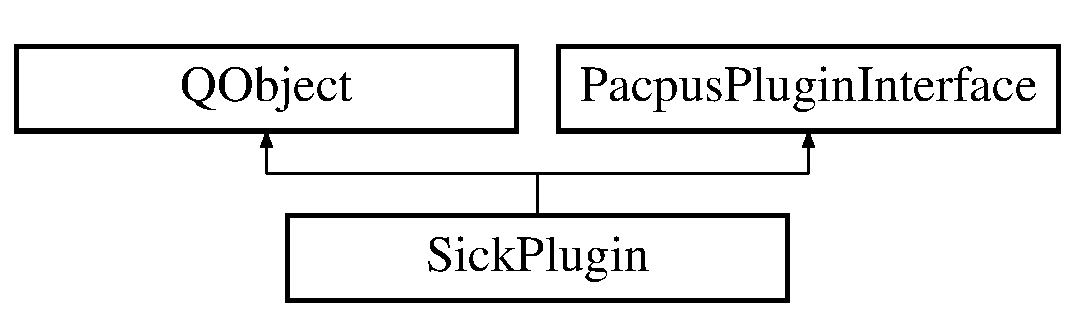
\includegraphics[height=2.000000cm]{classSickPlugin}
\end{center}
\end{figure}
\subsection*{Protected Member Functions}
\begin{DoxyCompactItemize}
\item 
\hypertarget{classSickPlugin_a8798b88aed6dfed590dda0c96a754dd0}{Q\-String {\bfseries name} ()}\label{classSickPlugin_a8798b88aed6dfed590dda0c96a754dd0}

\end{DoxyCompactItemize}


\subsection{Detailed Description}
Auto-\/generated plugin class. 

The documentation for this class was generated from the following files\-:\begin{DoxyCompactItemize}
\item 
Sick\-Plugin.\-h\item 
Sick\-Plugin.\-cpp\end{DoxyCompactItemize}

\hypertarget{classpacpus_1_1SickSocket}{\section{pacpus\-:\-:Sick\-Socket Class Reference}
\label{classpacpus_1_1SickSocket}\index{pacpus\-::\-Sick\-Socket@{pacpus\-::\-Sick\-Socket}}
}


The \hyperlink{classpacpus_1_1SickSocket}{Sick\-Socket} class Handles the ethernet connection with the remote sensor.  




{\ttfamily \#include $<$Sick\-Socket.\-h$>$}

Inheritance diagram for pacpus\-:\-:Sick\-Socket\-:\begin{figure}[H]
\begin{center}
\leavevmode
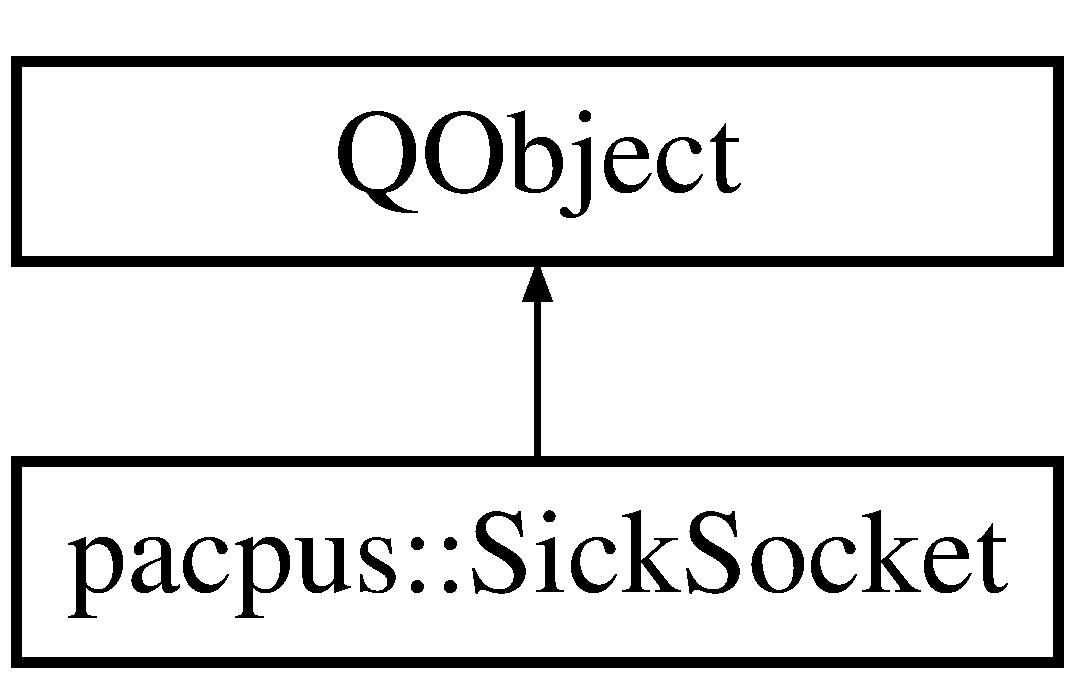
\includegraphics[height=2.000000cm]{classpacpus_1_1SickSocket}
\end{center}
\end{figure}
\subsection*{Public Slots}
\begin{DoxyCompactItemize}
\item 
\hypertarget{classpacpus_1_1SickSocket_a922b5337d2eae8ae855720f781743833}{void \hyperlink{classpacpus_1_1SickSocket_a922b5337d2eae8ae855720f781743833}{connect\-To\-Server} (Q\-String host, int port)}\label{classpacpus_1_1SickSocket_a922b5337d2eae8ae855720f781743833}

\begin{DoxyCompactList}\small\item\em Enable the connection to the server. \end{DoxyCompactList}\item 
\hypertarget{classpacpus_1_1SickSocket_a8fb9f7cb3f60287b65aaef6cd850238c}{int \hyperlink{classpacpus_1_1SickSocket_a8fb9f7cb3f60287b65aaef6cd850238c}{socket\-Connected} ()}\label{classpacpus_1_1SickSocket_a8fb9f7cb3f60287b65aaef6cd850238c}

\begin{DoxyCompactList}\small\item\em Warns about connection of the socket and launch configuration of the socket. \end{DoxyCompactList}\item 
void \hyperlink{classpacpus_1_1SickSocket_ae839a7cf980638e2217a26b1580bd136}{socket\-Ready\-Read} ()
\item 
\hypertarget{classpacpus_1_1SickSocket_a472586eeb677eddb03551c1938078d45}{void \hyperlink{classpacpus_1_1SickSocket_a472586eeb677eddb03551c1938078d45}{close\-Socket} ()}\label{classpacpus_1_1SickSocket_a472586eeb677eddb03551c1938078d45}

\begin{DoxyCompactList}\small\item\em Close the connection with the server. \end{DoxyCompactList}\item 
void \hyperlink{classpacpus_1_1SickSocket_afde0ecc1860a02c55ff6d7964cdf7a3c}{send\-To\-Server} (Q\-String data)
\begin{DoxyCompactList}\small\item\em send\-To\-Server Sends data to the remote lidar. \end{DoxyCompactList}\end{DoxyCompactItemize}
\subsection*{Signals}
\begin{DoxyCompactItemize}
\item 
\hypertarget{classpacpus_1_1SickSocket_a9fdf4483ca1b800cba3bbf1f2086edce}{void \hyperlink{classpacpus_1_1SickSocket_a9fdf4483ca1b800cba3bbf1f2086edce}{configuration} ()}\label{classpacpus_1_1SickSocket_a9fdf4483ca1b800cba3bbf1f2086edce}

\begin{DoxyCompactList}\small\item\em Asked for configuring sensor. \end{DoxyCompactList}\end{DoxyCompactItemize}
\subsection*{Public Member Functions}
\begin{DoxyCompactItemize}
\item 
\hypertarget{classpacpus_1_1SickSocket_ab866c3615462372f1a1fa790a300c1d7}{\hyperlink{classpacpus_1_1SickSocket_ab866c3615462372f1a1fa790a300c1d7}{Sick\-Socket} (\hyperlink{classpacpus_1_1AbstractSickSensor}{Abstract\-Sick\-Sensor} $\ast$parent)}\label{classpacpus_1_1SickSocket_ab866c3615462372f1a1fa790a300c1d7}

\begin{DoxyCompactList}\small\item\em Constructor. \end{DoxyCompactList}\item 
\hypertarget{classpacpus_1_1SickSocket_adca7f170e3fe00352175019703afdd6c}{\hyperlink{classpacpus_1_1SickSocket_adca7f170e3fe00352175019703afdd6c}{$\sim$\-Sick\-Socket} ()}\label{classpacpus_1_1SickSocket_adca7f170e3fe00352175019703afdd6c}

\begin{DoxyCompactList}\small\item\em Destructor. \end{DoxyCompactList}\end{DoxyCompactItemize}
\subsection*{Protected Slots}
\begin{DoxyCompactItemize}
\item 
void \hyperlink{classpacpus_1_1SickSocket_acb35dc2896ba2e6f4e4bc749f04fc71a}{socket\-Connection\-Closed} ()
\begin{DoxyCompactList}\small\item\em Says to the user the connection is closed. \end{DoxyCompactList}\item 
\hypertarget{classpacpus_1_1SickSocket_aea9be9bcfc97681ed665cf4095f351cb}{void \hyperlink{classpacpus_1_1SickSocket_aea9be9bcfc97681ed665cf4095f351cb}{socket\-Error} (Q\-Abstract\-Socket\-::\-Socket\-Error e)}\label{classpacpus_1_1SickSocket_aea9be9bcfc97681ed665cf4095f351cb}

\begin{DoxyCompactList}\small\item\em Warns the user an error occured. \end{DoxyCompactList}\end{DoxyCompactItemize}


\subsection{Detailed Description}
The \hyperlink{classpacpus_1_1SickSocket}{Sick\-Socket} class Handles the ethernet connection with the remote sensor. 

\subsection{Member Function Documentation}
\hypertarget{classpacpus_1_1SickSocket_afde0ecc1860a02c55ff6d7964cdf7a3c}{\index{pacpus\-::\-Sick\-Socket@{pacpus\-::\-Sick\-Socket}!send\-To\-Server@{send\-To\-Server}}
\index{send\-To\-Server@{send\-To\-Server}!pacpus::SickSocket@{pacpus\-::\-Sick\-Socket}}
\subsubsection[{send\-To\-Server}]{\setlength{\rightskip}{0pt plus 5cm}void pacpus\-::\-Sick\-Socket\-::send\-To\-Server (
\begin{DoxyParamCaption}
\item[{Q\-String}]{data}
\end{DoxyParamCaption}
)\hspace{0.3cm}{\ttfamily [slot]}}}\label{classpacpus_1_1SickSocket_afde0ecc1860a02c55ff6d7964cdf7a3c}


send\-To\-Server Sends data to the remote lidar. 


\begin{DoxyParams}{Parameters}
{\em data} & Data to be sent, translated in A\-S\-C\-I\-I. \\
\hline
\end{DoxyParams}
\hypertarget{classpacpus_1_1SickSocket_acb35dc2896ba2e6f4e4bc749f04fc71a}{\index{pacpus\-::\-Sick\-Socket@{pacpus\-::\-Sick\-Socket}!socket\-Connection\-Closed@{socket\-Connection\-Closed}}
\index{socket\-Connection\-Closed@{socket\-Connection\-Closed}!pacpus::SickSocket@{pacpus\-::\-Sick\-Socket}}
\subsubsection[{socket\-Connection\-Closed}]{\setlength{\rightskip}{0pt plus 5cm}void pacpus\-::\-Sick\-Socket\-::socket\-Connection\-Closed (
\begin{DoxyParamCaption}
{}
\end{DoxyParamCaption}
)\hspace{0.3cm}{\ttfamily [protected]}, {\ttfamily [slot]}}}\label{classpacpus_1_1SickSocket_acb35dc2896ba2e6f4e4bc749f04fc71a}


Says to the user the connection is closed. 

protected slot \hypertarget{classpacpus_1_1SickSocket_ae839a7cf980638e2217a26b1580bd136}{\index{pacpus\-::\-Sick\-Socket@{pacpus\-::\-Sick\-Socket}!socket\-Ready\-Read@{socket\-Ready\-Read}}
\index{socket\-Ready\-Read@{socket\-Ready\-Read}!pacpus::SickSocket@{pacpus\-::\-Sick\-Socket}}
\subsubsection[{socket\-Ready\-Read}]{\setlength{\rightskip}{0pt plus 5cm}void pacpus\-::\-Sick\-Socket\-::socket\-Ready\-Read (
\begin{DoxyParamCaption}
{}
\end{DoxyParamCaption}
)\hspace{0.3cm}{\ttfamily [slot]}}}\label{classpacpus_1_1SickSocket_ae839a7cf980638e2217a26b1580bd136}
Called when incoming data is received. Create an event and send it to the sensor's handler. \begin{DoxySeeAlso}{See Also}
Abstract\-Sick\-Component 
\end{DoxySeeAlso}


The documentation for this class was generated from the following files\-:\begin{DoxyCompactItemize}
\item 
Sick\-Socket.\-h\item 
Sick\-Socket.\-cpp\end{DoxyCompactItemize}

%--- End generated contents ---

% Index
\newpage
\phantomsection
\addcontentsline{toc}{chapter}{Index}
\printindex

\end{document}
